% Options for packages loaded elsewhere
\PassOptionsToPackage{unicode}{hyperref}
\PassOptionsToPackage{hyphens}{url}
\documentclass[
  11pt,
  fontset=fandol]{ctexart}
\usepackage{xcolor}
\usepackage[a4paper,margin=22mm]{geometry}
\usepackage{amsmath,amssymb}
\setcounter{secnumdepth}{-\maxdimen} % remove section numbering
\usepackage{iftex}
\ifPDFTeX
  \usepackage[T1]{fontenc}
  \usepackage[utf8]{inputenc}
  \usepackage{textcomp} % provide euro and other symbols
\else % if luatex or xetex
  \usepackage{unicode-math} % this also loads fontspec
  \defaultfontfeatures{Scale=MatchLowercase}
  \defaultfontfeatures[\rmfamily]{Ligatures=TeX,Scale=1}
\fi
\usepackage{lmodern}
\ifPDFTeX\else
  % xetex/luatex font selection
\fi
% Use upquote if available, for straight quotes in verbatim environments
\IfFileExists{upquote.sty}{\usepackage{upquote}}{}
\IfFileExists{microtype.sty}{% use microtype if available
  \usepackage[]{microtype}
  \UseMicrotypeSet[protrusion]{basicmath} % disable protrusion for tt fonts
}{}
\makeatletter
\@ifundefined{KOMAClassName}{% if non-KOMA class
  \IfFileExists{parskip.sty}{%
    \usepackage{parskip}
  }{% else
    \setlength{\parindent}{0pt}
    \setlength{\parskip}{6pt plus 2pt minus 1pt}}
}{% if KOMA class
  \KOMAoptions{parskip=half}}
\makeatother
\usepackage{longtable,booktabs,array}
\newcounter{none} % for unnumbered tables
\usepackage{calc} % for calculating minipage widths
% Correct order of tables after \paragraph or \subparagraph
\usepackage{etoolbox}
\makeatletter
\patchcmd\longtable{\par}{\if@noskipsec\mbox{}\fi\par}{}{}
\makeatother
% Allow footnotes in longtable head/foot
\IfFileExists{footnotehyper.sty}{\usepackage{footnotehyper}}{\usepackage{footnote}}
\makesavenoteenv{longtable}
\setlength{\emergencystretch}{3em} % prevent overfull lines
\providecommand{\tightlist}{%
  \setlength{\itemsep}{0pt}\setlength{\parskip}{0pt}}
\usepackage{float,caption,tikz,pgfplots}
\usepgfplotslibrary{groupplots}
\pgfplotsset{compat=1.18}
\setlength{\parskip}{.45em}
\setlength{\parindent}{0pt}
\setlength{\emergencystretch}{3em}
\pagestyle{plain}
\usepackage{bookmark}
\IfFileExists{xurl.sty}{\usepackage{xurl}}{} % add URL line breaks if available
\urlstyle{same}
\hypersetup{
  pdftitle={细胞核中心定位：实验结果与逐个细胞核分析------阶段报告 8},
  pdfauthor={bdd26 research},
  hidelinks,
  pdfcreator={LaTeX via pandoc}}

\title{细胞核中心定位：实验结果与逐个细胞核分析------阶段报告 8}
\author{bdd26 research}
\date{17 November 2026}

\begin{document}
\maketitle

{
\setcounter{tocdepth}{2}
\tableofcontents
\newpage
}
\subsection{研究问题与本阶段结论}\label{ux7814ux7a76ux95eeux9898ux4e0eux672cux9636ux6bb5ux7ed3ux8bba}

阶段报告 7 介绍至 P26。本报告从 P27 开始，依次说明 P27 至 P31
的研究问题、对照、训练与开发评估结果，以及固定图像中的具体细胞核变化。图像编码器是从图像中提取特征的模型部分。P27--P30
比较预训练图像编码器中不同层的训练位置；P31
保持编码器后十二层训练，在预测细胞核中心的检测头中加入分组归一化。

五轮实验使用 PanNuke 第一折内的 2,134 张训练图像和另外 522
张开发评估图像。后者包含 12,250 个标注细胞核，其中 145 个死亡细胞核位于
11 张图像内，且轮廓不接触图像边缘；32 个的面积小于 67
平方像素。预测中心与标注中心在三像素内一对一匹配。检出率是匹配标注数除以标注总数；匹配精度是匹配点数除以预测点总数；额外预测点是未匹配的预测。区间通过按组织类别对同一批图像重复抽样、计算两方案差值得到。每轮对照与实验各用随机种子
19、1 独立训练 130
轮。随机种子控制训练过程的随机选择，评估使用最后一轮模型。训练图像与开发评估图像的角色始终保持区分。

两种子下，P27 多找到 6／15 个死亡核，P28 变化 +2／−1，P29 增加
16／13，P30 增加 7／15，P31 增加 8／2。P30 的总体匹配增加
648／516，同时额外点减少 215／254；P31 的总体匹配变化为
−140／+6。每一轮均与自己同种子的对照比较，下图将这五轮并列；逐图分析说明这些净变化由哪些新增和丢失组成。

\begin{figure}[H]\centering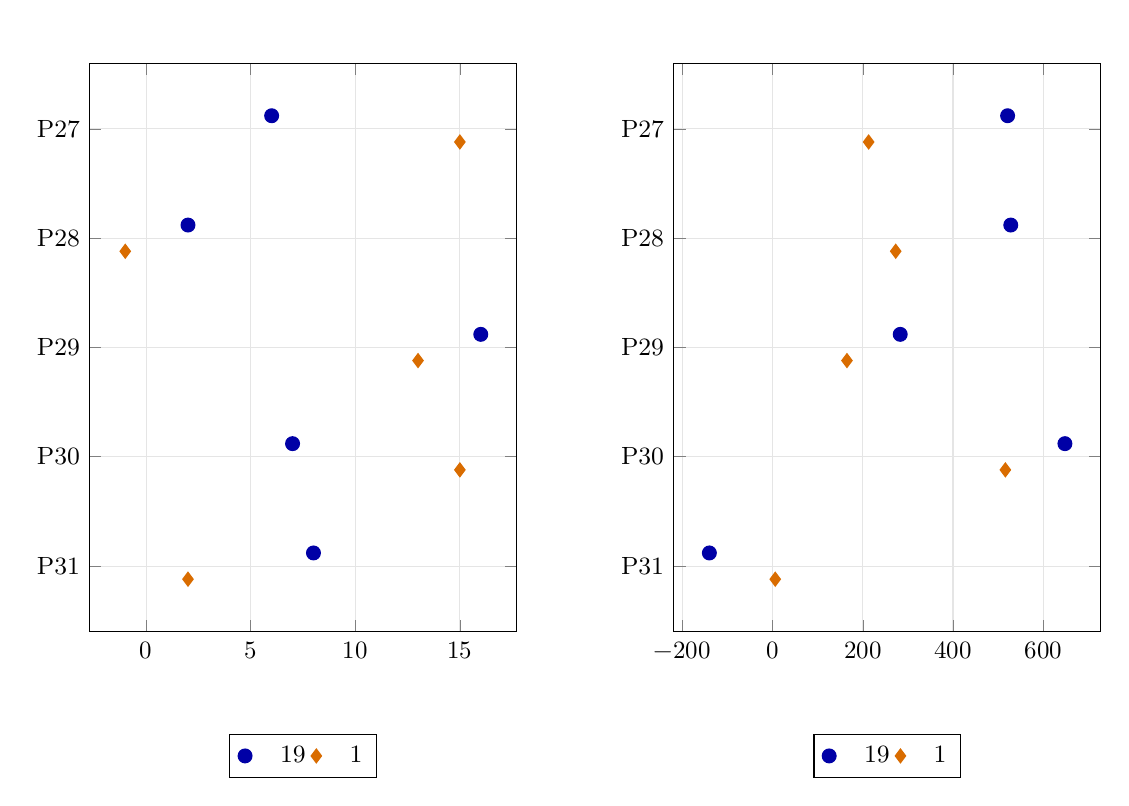
\begin{tikzpicture}
\begin{groupplot}[group style={group size=2 by 1,horizontal sep=2.0cm},width=7cm,height=8.8cm,ytick={0,1,2,3,4},yticklabels={P27,P28,P29,P30,P31},ymin=-.6,ymax=4.6,y dir=reverse,grid=major,grid style={gray!20},tick label style={font=\small},label style={font=\small},title style={font=\small},legend style={font=\small,at={(.5,-.18)},anchor=north,legend columns=2}]
\nextgroupplot[title={死亡细胞核匹配变化},xlabel={新方案减同轮对照：匹配数}]
\addplot[only marks,mark=*,mark size=2.5pt,color=blue!65!black] coordinates {(6,-0.12) (2,0.88) (16,1.88) (7,2.88) (8,3.88)};
\addlegendentry{种子 19}
\addplot[only marks,mark=diamond*,mark size=2.5pt,color=orange!85!black] coordinates {(15,0.12) (-1,1.12) (13,2.12) (15,3.12) (2,4.12)};
\addlegendentry{种子 1}
\nextgroupplot[title={全部细胞核匹配变化},xlabel={新方案减同轮对照：匹配数}]
\addplot[only marks,mark=*,mark size=2.5pt,color=blue!65!black] coordinates {(521,-0.12) (528,0.88) (283,1.88) (648,2.88) (-140,3.88)};
\addlegendentry{种子 19}
\addplot[only marks,mark=diamond*,mark size=2.5pt,color=orange!85!black] coordinates {(213,0.12) (273,1.12) (165,2.12) (516,3.12) (6,4.12)};
\addlegendentry{种子 1}
\end{groupplot}
\end{tikzpicture}
\caption{P27–P31 各实验方案相对同轮对照的变化。左：找到的死亡细胞核数；右：找到的全部细胞核数。圆点与菱形分别代表种子 19 和 1。}\end{figure}

\subsection{P27：训练前十二层}\label{p27ux8badux7ec3ux524dux5341ux4e8cux5c42}

对照训练编码器最后十二层；实验组改为训练前十二层。两组可训练的编码器参数数量相同，其余数据、学习率和检测方法保持一致。

{\def\LTcaptype{none} % do not increment counter
\begin{longtable}[]{@{}
  >{\raggedright\arraybackslash}p{(\linewidth - 10\tabcolsep) * \real{0.1304}}
  >{\raggedleft\arraybackslash}p{(\linewidth - 10\tabcolsep) * \real{0.1739}}
  >{\raggedleft\arraybackslash}p{(\linewidth - 10\tabcolsep) * \real{0.1739}}
  >{\raggedleft\arraybackslash}p{(\linewidth - 10\tabcolsep) * \real{0.1739}}
  >{\raggedleft\arraybackslash}p{(\linewidth - 10\tabcolsep) * \real{0.1739}}
  >{\raggedleft\arraybackslash}p{(\linewidth - 10\tabcolsep) * \real{0.1739}}@{}}
\toprule\noalign{}
\begin{minipage}[b]{\linewidth}\raggedright
种子与更新位置
\end{minipage} & \begin{minipage}[b]{\linewidth}\raggedleft
内部死亡核匹配
\end{minipage} & \begin{minipage}[b]{\linewidth}\raggedleft
小死亡核匹配
\end{minipage} & \begin{minipage}[b]{\linewidth}\raggedleft
总体匹配 / 标注
\end{minipage} & \begin{minipage}[b]{\linewidth}\raggedleft
总体精确率
\end{minipage} & \begin{minipage}[b]{\linewidth}\raggedleft
额外点
\end{minipage} \\
\midrule\noalign{}
\endhead
\bottomrule\noalign{}
\endlastfoot
19，后 12 块 & 72/145 & 10/32 & 7,264/12,250 & 69.41\% & 3,202 \\
19，前 12 块 & 78/145 & 9/32 & 7,785/12,250 & 74.25\% & 2,700 \\
1，后 12 块 & 65/145 & 6/32 & 7,395/12,250 & 69.49\% & 3,247 \\
1，前 12 块 & 80/145 & 10/32 & 7,608/12,250 & 74.89\% & 2,551 \\
\end{longtable}
}

种子 19 的总输出点只增加 19 个，同时多配对 521 个核。种子 1 少输出 483
个点，同时多配对 213
个核。两组变化都显示输出点与标注位置的配对改善。训练集总体召回从
97.72\%/97.89\% 降至 88.80\%/87.82\%，最终中心预测损失从 0.0563/0.0574
升至
0.2643/0.2507。前层更新组在训练集上的覆盖更低，在本开发评估集上的覆盖更高。冻结后半段仍需将梯度传回前半段，观察到的训练过程耗时增加
21\%/23\%，分配显存峰值从 4.05 增至 4.84 GiB。

两种子死亡核召回增加 4.14/10.34 个百分点。按组织分层、对图像配对重采样的
95\% 区间为 −0.57 至 +15.38 和 +1.85 至 +15.49
个百分点。依次删除任意一张含死亡核图像后，增益范围仍为 +2.31 至 +10.42
和 +8.46 至 +14.17 个百分点。前层组绝对死亡核召回为
53.79\%/55.17\%，总体精确率为 74.25\%/74.89\%。原判定要求分别达到 60\%
和 75\%，两种子均未满足完整判定。关闭本次固定前 12
块设置。数据来自反复用于方法开发的第 1 折评估集。

\subsubsection{哪些图像和对象发生改变}\label{ux54eaux4e9bux56feux50cfux548cux5bf9ux8c61ux53d1ux751fux6539ux53d8}

宫颈组织图像 1756 净增 3/4，食管组织图像 2076 净增 2/2，肺组织合计净增
3/3。含 49 个内部死亡核的结肠组织图像 1482，在种子 19 从 17 降到
13，在种子 1 从 10 升到 16。固定八张图的 53 个内部死亡核中，种子 19 保留
26、找回 11、丢失 7、两组都漏 9。种子 1 分别为 26、6、7、14。该子集净增
4、净减 1；种子 1 的总体净增主要来自固定示例以外的图像。

\noindent

\begin{minipage}{\linewidth}\centering
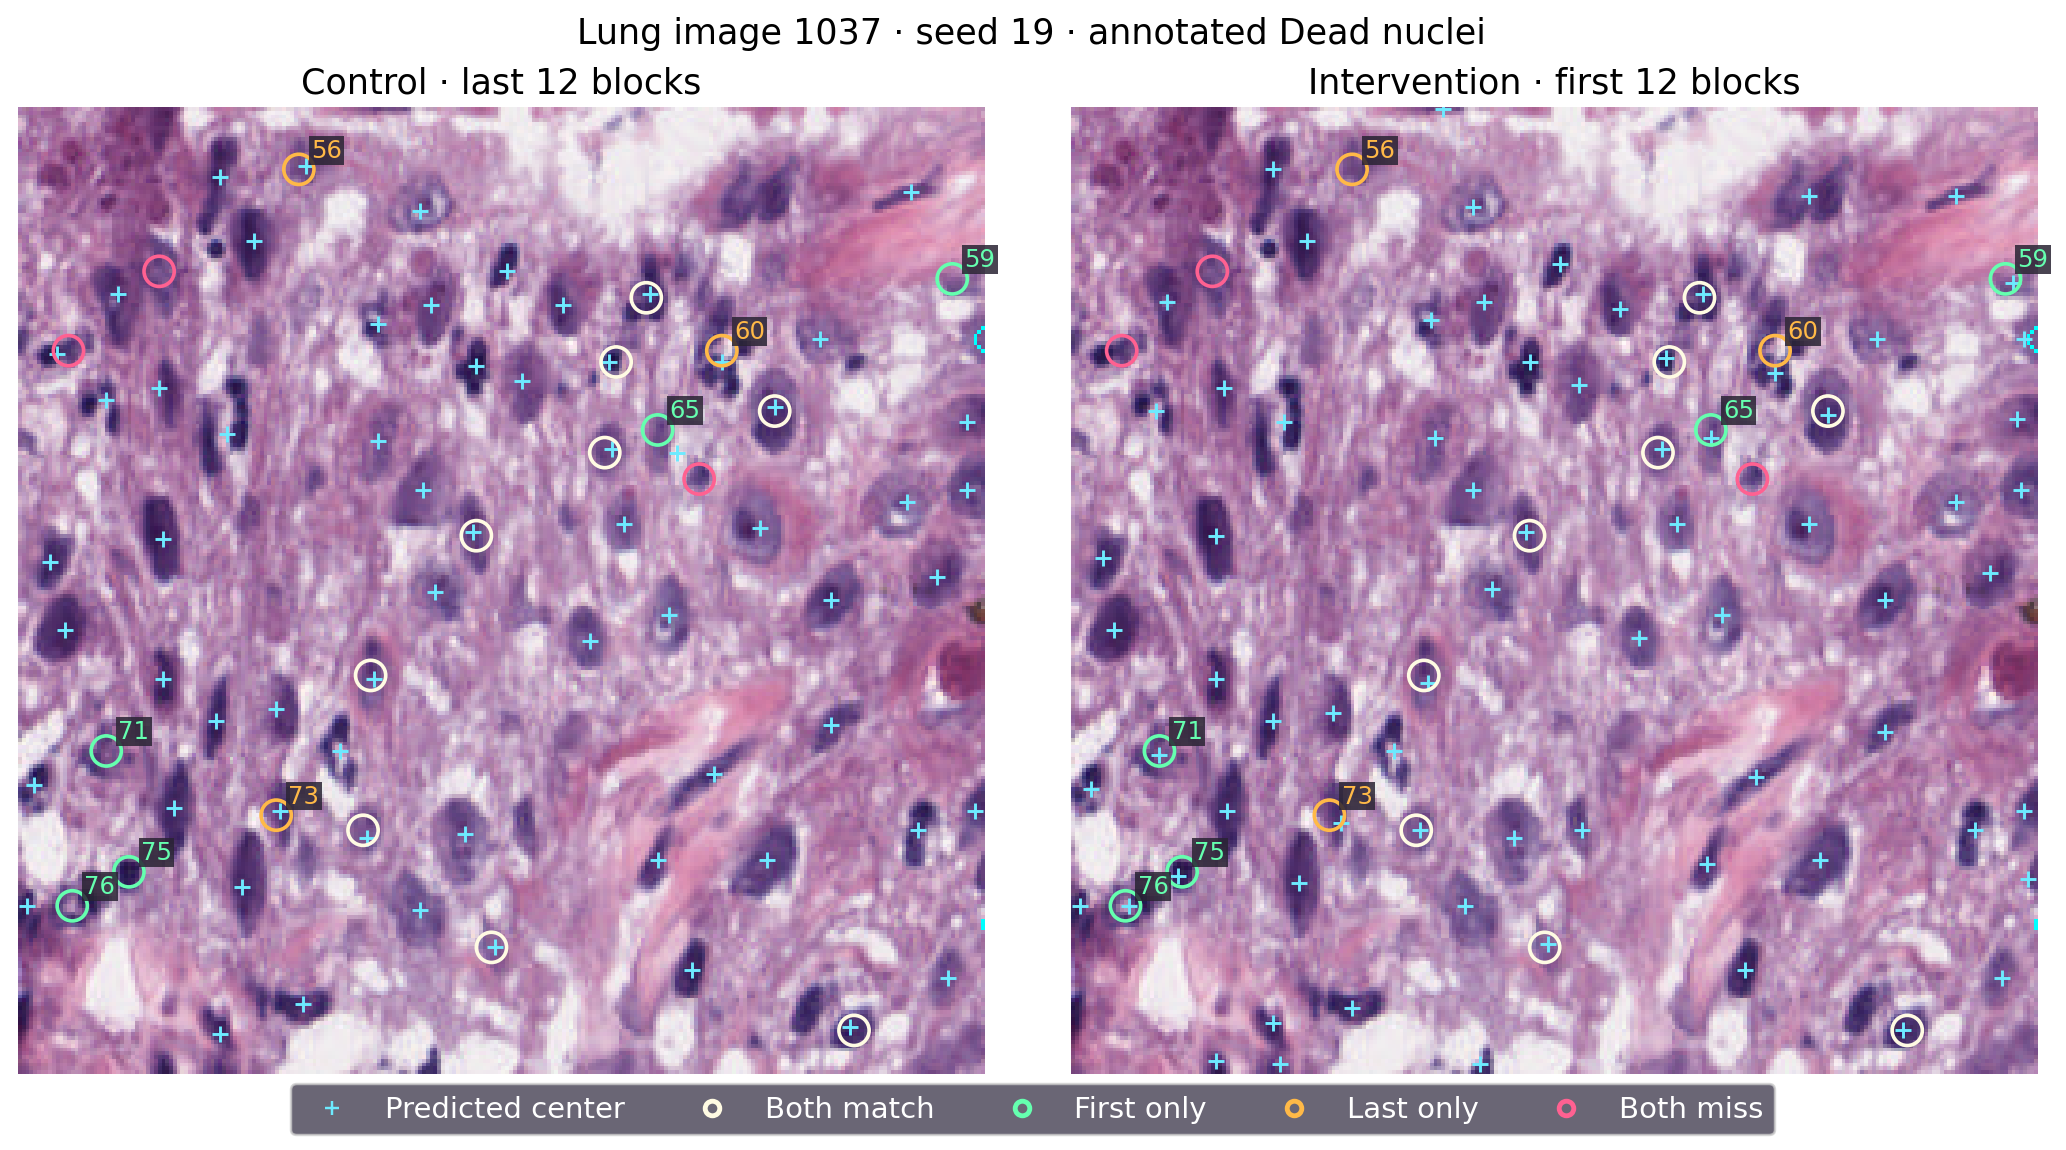
\includegraphics[width=\linewidth,height=.40\textheight,keepaspectratio]{assets/p27_image_1037_seed_19.png}
\captionof{figure}{肺组织图像 1037，种子 19。种子 19；左为后十二层对照，右为前十二层方案。青色十字为预测中心；白、绿、橙、粉圆圈分别表示共同找到、仅新方案找到、仅对照找到和共同漏检}
\raggedright

青色十字标出所有预测的细胞核中心。圆圈标出内部死亡核标注，两幅图重复相同的圆圈颜色来表示两组共同的配对结局。图像 1037 的种子 19 从 12/20 增至 14/20，实际找回 5 个并丢失 3 个。对象 65 的标注中心为（85，169，先行后列），处于图像中央深染组织边缘，最近输出点从 7.81 像素缩至 2.00 像素，形成匹配。左下方对象 71（170，23）从 21.02 像素缩至 1.00 像素。左上方对象 56（16，74）从 2.24 像素增至 21.00 像素，附近缺少输出点。下部对象 73（187，68）从 1.41 增至 3.61 像素，越过了半径界线。

\end{minipage}

\noindent

\begin{minipage}{\linewidth}\centering
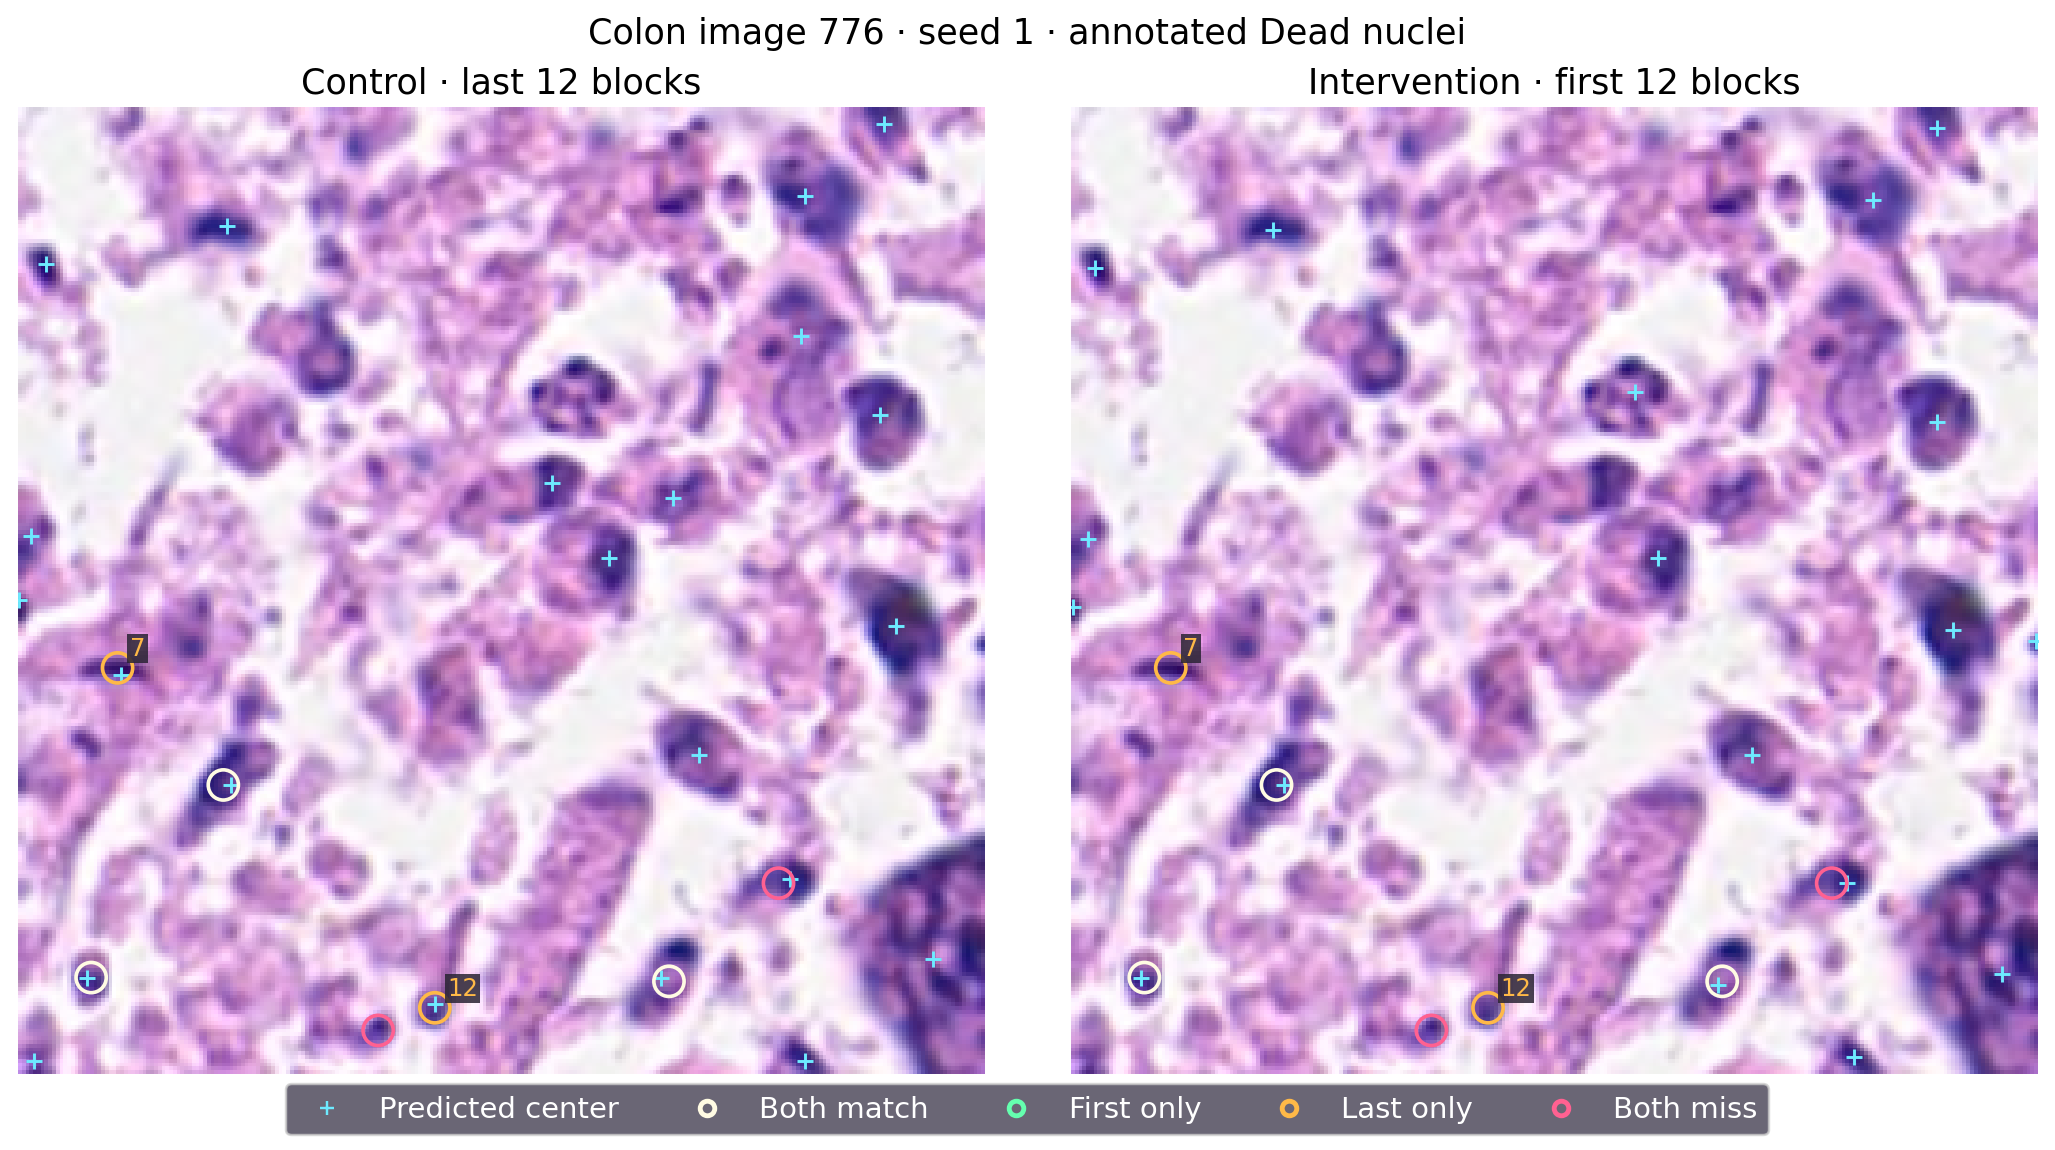
\includegraphics[width=\linewidth,height=.40\textheight,keepaspectratio]{assets/p27_image_776_seed_1.png}
\captionof{figure}{结肠组织图像 776，种子 1。种子 1；左为后十二层对照，右为前十二层方案。青色十字为预测中心；白、绿、橙、粉圆圈分别表示共同找到、仅新方案找到、仅对照找到和共同漏检}
\raggedright

图像 776 的种子 1 从 5/7 降到 3/7。对象 7（148，26）和对象 12（238，110）的最近输出距离分别从 2.24 增至 30.53、从 1.00 增至 61.29 像素。两者均表现为近处缺少解码后的预测点。对象 8（179，54）在两组都匹配到（179，56）。右下部对象 9（205，201）两组都有肉眼可见的近处十字，距离分别为 3.16 和 4.00 像素，均在半径外。坐标可以区分临界位置偏差与附近无输出。区分预测分数弱、峰位置偏移和峰值筛选的影响，需要保留完整分数图。

\end{minipage}

\subsection{P28：交错训练十二层}\label{p28ux4ea4ux9519ux8badux7ec3ux5341ux4e8cux5c42}

对照训练编码器最后十二层；实验组训练从零开始编号为 1、3、5 至 23
的十二层，即隔一层训练一层。两组可训练编码器参数数量相同。

{\def\LTcaptype{none} % do not increment counter
\begin{longtable}[]{@{}
  >{\raggedright\arraybackslash}p{(\linewidth - 10\tabcolsep) * \real{0.1304}}
  >{\raggedleft\arraybackslash}p{(\linewidth - 10\tabcolsep) * \real{0.1739}}
  >{\raggedleft\arraybackslash}p{(\linewidth - 10\tabcolsep) * \real{0.1739}}
  >{\raggedleft\arraybackslash}p{(\linewidth - 10\tabcolsep) * \real{0.1739}}
  >{\raggedleft\arraybackslash}p{(\linewidth - 10\tabcolsep) * \real{0.1739}}
  >{\raggedleft\arraybackslash}p{(\linewidth - 10\tabcolsep) * \real{0.1739}}@{}}
\toprule\noalign{}
\begin{minipage}[b]{\linewidth}\raggedright
种子、设置
\end{minipage} & \begin{minipage}[b]{\linewidth}\raggedleft
内部死亡细胞核
\end{minipage} & \begin{minipage}[b]{\linewidth}\raggedleft
小型死亡细胞核
\end{minipage} & \begin{minipage}[b]{\linewidth}\raggedleft
全部匹配
\end{minipage} & \begin{minipage}[b]{\linewidth}\raggedleft
精度
\end{minipage} & \begin{minipage}[b]{\linewidth}\raggedleft
额外点
\end{minipage} \\
\midrule\noalign{}
\endhead
\bottomrule\noalign{}
\endlastfoot
19, 后 12 层 & 68/145 & 7/32 & 7177/12,250 & 69.23\% & 3190 \\
19, 奇数编号 12 层 & 70/145 & 9/32 & 7705/12,250 & 71.24\% & 3110 \\
1, 后 12 层 & 72/145 & 10/32 & 7361/12,250 & 69.07\% & 3296 \\
1, 奇数编号 12 层 & 71/145 & 9/32 & 7634/12,250 & 72.44\% & 2905 \\
\end{longtable}
}

总体召回增加 4.31/2.23 个百分点，精度增加 2.01/3.36 个百分点。种子 19
预测点增加 448 而匹配增加 528，说明新增点与既有点合计更有效；种子 1
预测点减少 118 而匹配增加
273，说明更少的点找到更多核。小型死亡细胞核分别 7→9、10→9。

两个种子的训练集检出率分别从 97.91\% 降至 96.32\%，从 97.89\% 降至
96.31\%。最终中心检测损失分别从 0.05339 升至 0.08767，从 0.05474 升至
0.08310。对照训练耗时 4.009/4.020 小时，交错层耗时 4.781/4.757
小时，增加 19.27\%/18.33\%；峰值已分配显存从 4.05 增至 4.78
GiB。四任务调度总耗时 18:19:46，即 18.3294 GPU
小时，包含启动、检查点和保存时间。

原有图像级自助抽样与保存的判定函数已分别复算并一致。死亡细胞核召回变化为+1.38/−0.69
个百分点，95\%
区间为{[}−6.29,+13.27{]}/{[}−2.54,+2.34{]}。最终死亡细胞核召回
48.28\%/48.97\%，提升幅度、区间下界以及精度
71.24\%/72.44\%均未满足固定条件，两种子完整判定均失败，关闭具体奇数层方案。

\subsubsection{组织分布与逐对象解释}\label{ux7ec4ux7ec7ux5206ux5e03ux4e0eux9010ux5bf9ux8c61ux89e3ux91ca}

肺组织合计变化+6/0，结肠−4/−1。种子 19 肺组织图 1038 增加 5 个，而结肠图
1482 减少 4 个。结肠图 1482 拥有 49/145，即
33.79\%的内部死亡细胞核标注，贡献集中。仅作敏感性分析时，删除该图会使种子
19 变化成为 6/96=6.25\%；删除肺组织图 1038 则为−3/130=−2.31\%。种子 1
逐张删除后的范围为−1.54\%至
0.00\%。实际判定保留全部十一张图，以上计算用于量化图像集中程度。

原先固定的八张样例包含 53 个内部死亡细胞核。种子 19
对照和实验方案共同找到 26 个、交错层新增 7 个、丢失 6 个、共同遗漏 14
个；种子 1 为
28、5、5、15。固定样例净变化+1/0，全体评估为+2/−1。样例用于解释具体位置的变化，全体
522 张图决定指标。

\noindent

\begin{minipage}{\linewidth}\centering
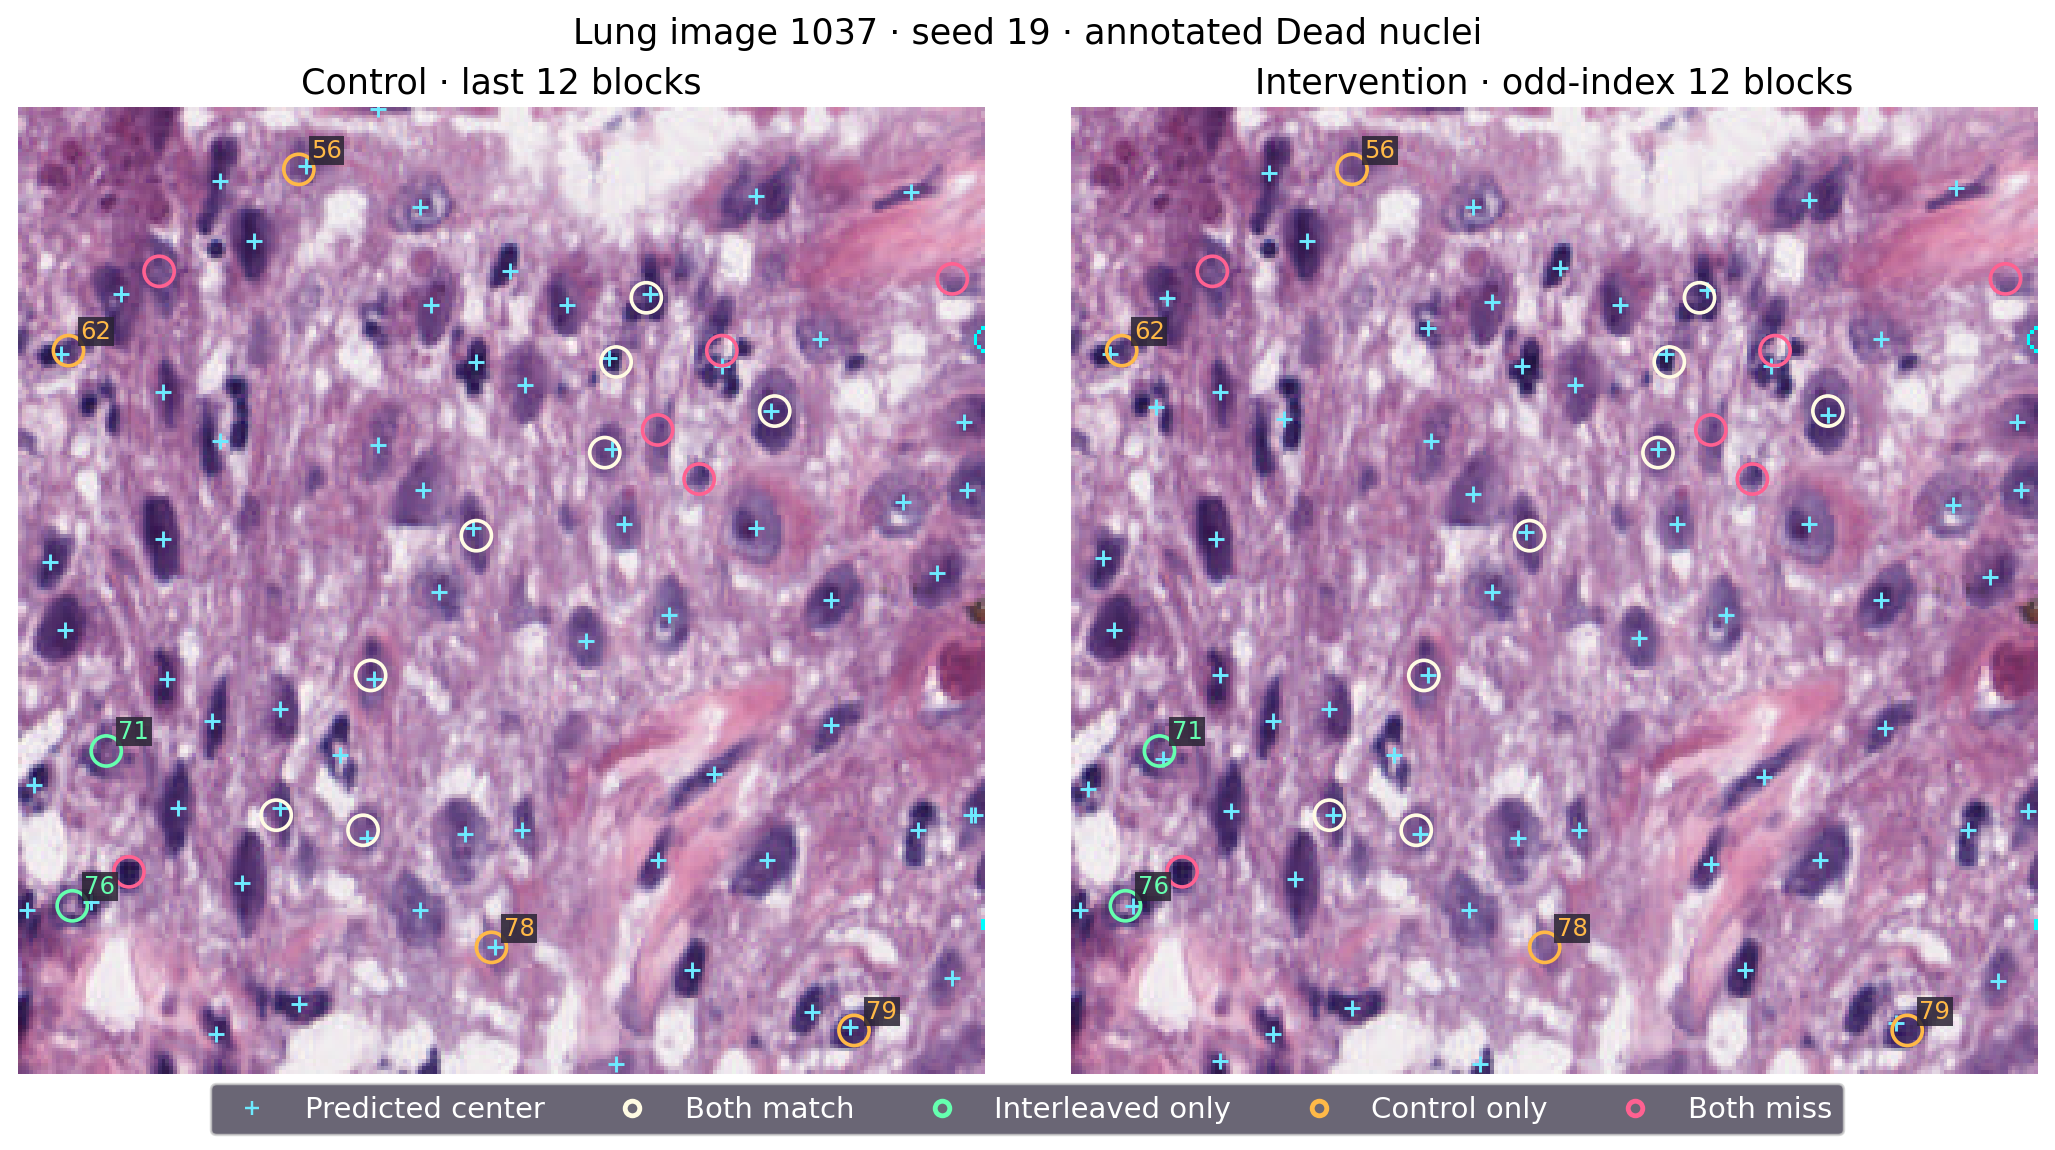
\includegraphics[width=\linewidth,height=.40\textheight,keepaspectratio]{assets/p28_image_1037_seed_19.png}
\captionof{figure}{肺组织图 1037、种子 19，左右使用相同对象颜色。种子 19；左为后十二层对照，右为交错十二层方案。青色十字为预测中心；白、绿、橙、粉圆圈分别表示共同找到、仅新方案找到、仅对照找到和共同漏检}
\raggedright

青色十字是全部预测点；白圈为对照和实验方案都匹配的死亡细胞核，绿圈为交错层新增，橙圈为对照找到而交错层丢失，粉圈为共同遗漏。编号对应保存的人工标注列表位置，坐标采用行、列，见对象表。同色圆圈在两面板中表示同一对象的成对结果。

\end{minipage}

肺组织图 1037 种子 19 从 12 个匹配变为 10 个，新增 2 个、丢失 4
个。左下对象 71 位于(170,23)，最近预测点距离 21.02→2.24 像素；对象 76
位于(211,14)，5.10→2.00。左上对象 56 位于(16,74)，2.24→22.02；靠下对象
78 位于(222,125)，1.00→22.36，交错层在这些标注附近没有输出点。对象 62
位于(64,13)，2.24→3.16；对象 79
位于(244,221)，1.41→3.61，这两次丢失位于三像素匹配边界，肉眼看似接近的点仍可超出匹配半径。

\noindent

\begin{minipage}{\linewidth}\centering
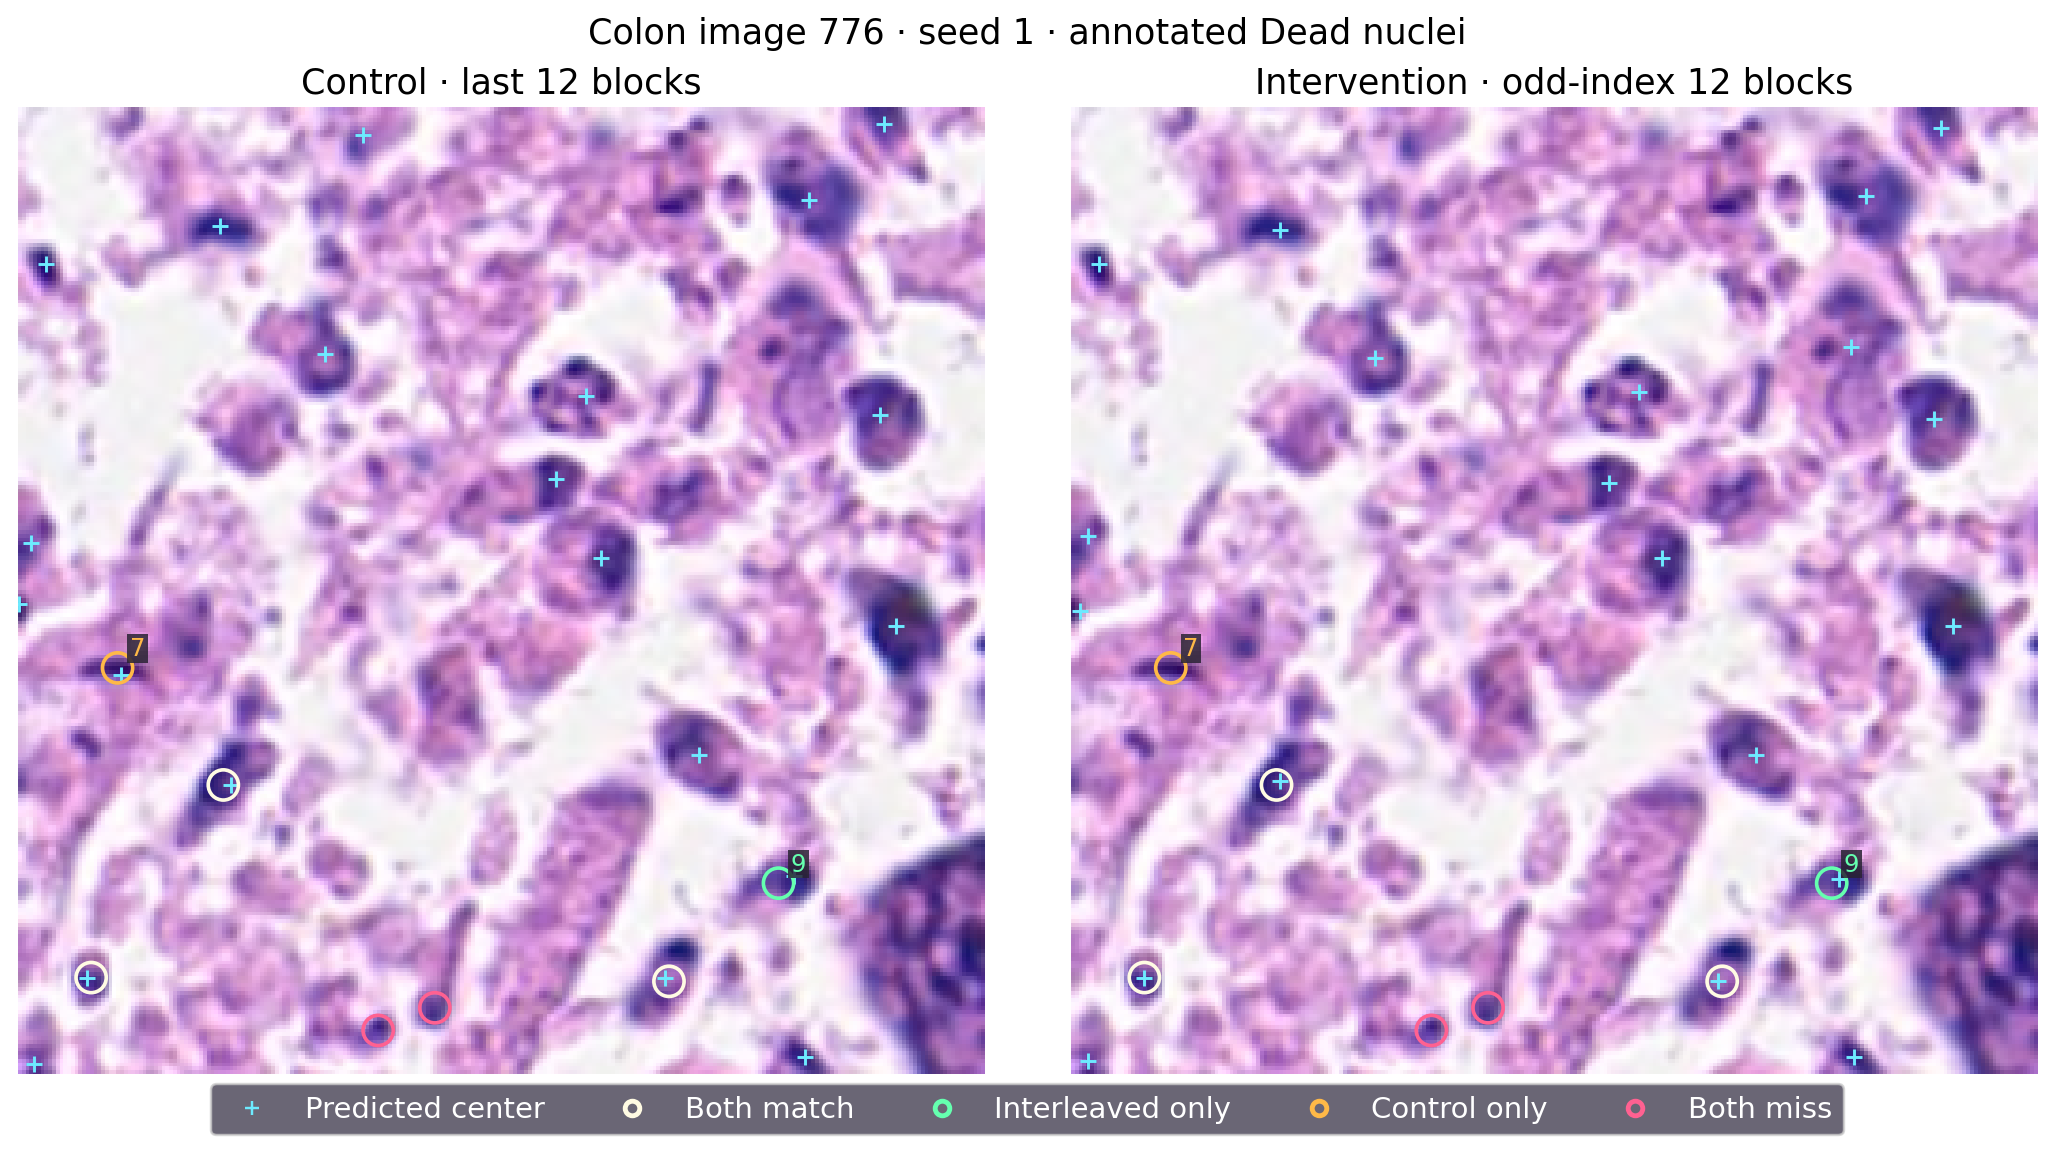
\includegraphics[width=\linewidth,height=.40\textheight,keepaspectratio]{assets/p28_image_776_seed_1.png}
\captionof{figure}{结肠图 776、种子 1：总数不变，但找到的对象发生交换。种子 1；左为后十二层对照，右为交错十二层方案。青色十字为预测中心；白、绿、橙、粉圆圈分别表示共同找到、仅新方案找到、仅对照找到和共同漏检}
\raggedright

结肠图 776 在两种子均保持 4/7 个匹配，却都新增一个、丢失一个。对象 7 位于(148,26)，对照距离 2.83/2.24 像素，交错层均为 28.30，附近的输出点消失。对象 9 位于(205,201)，交错层预测(204,203)，距离 2.24；对照距离为 3.16/4.47。总体相同的单图数值因此隐藏了“丢失一个远离输出的核、找回一个进入匹配邻域的核”的交换。

\end{minipage}

图中的深染轮廓、染色梯度与密集组织提供位置背景。坐标直接证明输出点的消失或偏移；要进一步区分标注附近预测分数不足、局部峰值偏移和筛选抑制，需要保存未筛选概率图。原始四面板PNG同时保留了中心响应预览。这些观察为后续机制测量提供对象位置，不直接指定内部表征原因。

\subsection{P29：训练前六层与后六层}\label{p29ux8badux7ec3ux524dux516dux5c42ux4e0eux540eux516dux5c42}

对照训练编码器最后十二层；实验组训练前六层和后六层，保持同样的可训练参数数量。

种子 19 的结果如下。

{\def\LTcaptype{none} % do not increment counter
\begin{longtable}[]{@{}
  >{\raggedright\arraybackslash}p{(\linewidth - 12\tabcolsep) * \real{0.1111}}
  >{\raggedleft\arraybackslash}p{(\linewidth - 12\tabcolsep) * \real{0.1481}}
  >{\raggedleft\arraybackslash}p{(\linewidth - 12\tabcolsep) * \real{0.1481}}
  >{\raggedleft\arraybackslash}p{(\linewidth - 12\tabcolsep) * \real{0.1481}}
  >{\raggedleft\arraybackslash}p{(\linewidth - 12\tabcolsep) * \real{0.1481}}
  >{\raggedleft\arraybackslash}p{(\linewidth - 12\tabcolsep) * \real{0.1481}}
  >{\raggedleft\arraybackslash}p{(\linewidth - 12\tabcolsep) * \real{0.1481}}@{}}
\toprule\noalign{}
\begin{minipage}[b]{\linewidth}\raggedright
更新范围
\end{minipage} & \begin{minipage}[b]{\linewidth}\raggedleft
内部死亡细胞核
\end{minipage} & \begin{minipage}[b]{\linewidth}\raggedleft
小型死亡细胞核
\end{minipage} & \begin{minipage}[b]{\linewidth}\raggedleft
全部匹配
\end{minipage} & \begin{minipage}[b]{\linewidth}\raggedleft
总召回
\end{minipage} & \begin{minipage}[b]{\linewidth}\raggedleft
精度
\end{minipage} & \begin{minipage}[b]{\linewidth}\raggedleft
未匹配预测
\end{minipage} \\
\midrule\noalign{}
\endhead
\bottomrule\noalign{}
\endlastfoot
最后十二层 & 65/145 & 7/32 & 7,257/12,250 & 59.24\% & 69.73\% & 3,150 \\
前六层＋后六层 & 81/145 & 11/32 & 7,540/12,250 & 61.55\% & 70.96\% &
3,085 \\
\end{longtable}
}

实验模型多输出 218 个点，却多匹配 283
个核，预测的有效性有所提高。内部死亡细胞核召回增加 11.0345
个百分点，原固定 1,000 次按组织分层的图像重采样区间为
［+3.0457，+27.9570］个百分点；总召回增加 2.3102 个百分点、精度增加
1.2328 个百分点。原种子级完整条件中，死亡细胞核召回 0.60 和精度 0.75
两项未满足，其余种子 19 条件均满足。种子 1 的内部死亡细胞核召回改善为
8.9655 个百分点，同样未满足两项绝对条件。

训练集总体召回从 97.51\% 降至 95.47\%，训练内部死亡细胞核覆盖从 630/656
降至 607/656。训练过程耗时为 4.0130/4.8652 小时，实验模型增加约
21.24\%；峰值已分配显存约为 4.05/4.84 GiB。种子 19 两项调度总耗时分别为
4:13:24 和
5:00:21，包含启动、评估和保存。训练覆盖、开发检测和调度成本分别回答不同的问题。

\subsubsection{哪些组织图像贡献了改善}\label{ux54eaux4e9bux7ec4ux7ec7ux56feux50cfux8d21ux732eux4e86ux6539ux5584}

六张图像增加匹配，一张减少，四张不变。肺组织净增加 4 个，结肠 3 个，宫颈
2 个，食管 5 个，胃 2 个；乳腺和子宫不变。肺组织图像 1038 和食管图像
2076 各增加 5 个，合计贡献 16 个净增量中的 10 个。肺组织图像 1025
则减少两个。结肠图像 1482 含 49/145 个目标对象，对照和实验方案均只匹配
13 个，该图仍有 36 个目标核未匹配。

逐一去掉一张 包含死亡细胞核的图像作敏感性分析后，召回改善范围为
8.03\%--16.67\%，均为正。种子 19
的改善符号因此不依赖单张图像。正式原判定仍包含全部十一张图像。只有一张包含死亡细胞核的图像的组织，提供的组织内跨图像一致性证据有限。

\subsubsection{固定样例中的逐核变化}\label{ux56faux5b9aux6837ux4f8bux4e2dux7684ux9010ux6838ux53d8ux5316}

预先固定的八张评估样例包含 53 个内部死亡细胞核。种子 19
中，对照和实验方案共同找到 30 个，实验模型新增 6 个、丢失 4 个，共同漏检
13 个，净增两个；完整 522 张评估图像的净增量为
16。对象编号和行、列坐标保存在
fixed\_objects.csv。青色十字是预测点；白、绿、橙、粉色圆圈依次表示共同找到、新增、丢失和共同漏检。

\noindent

\begin{minipage}{\linewidth}\centering
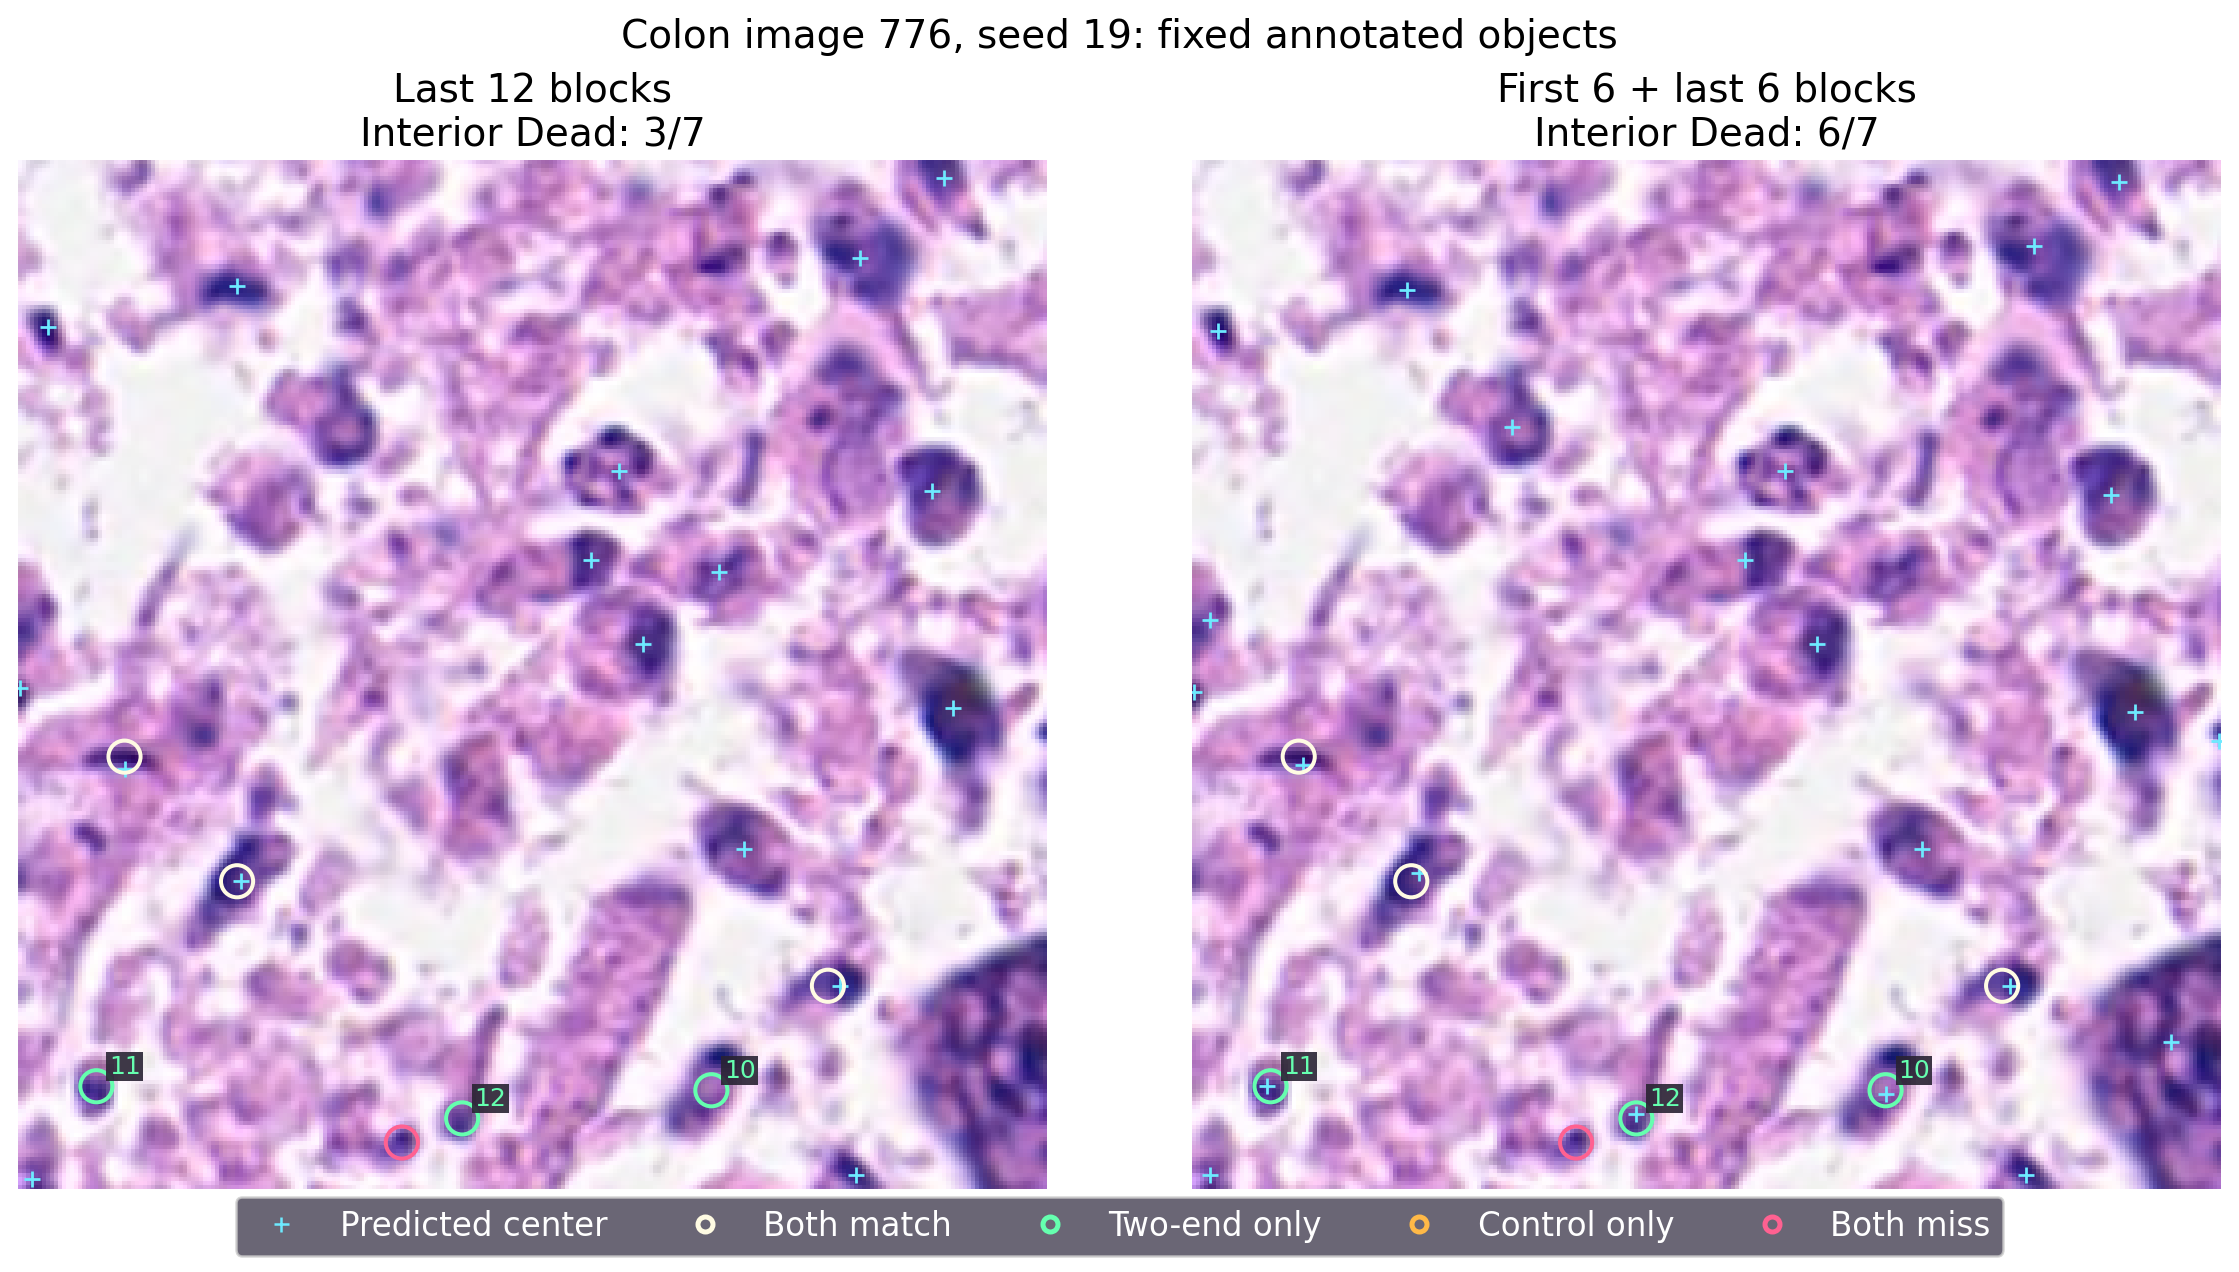
\includegraphics[width=\linewidth,height=.40\textheight,keepaspectratio]{assets/p29_image_776_seed_19.png}
\captionof{figure}{结肠图像 776：下方组织区域新增三个核。种子 19；左为后十二层对照，右为前六层加后六层方案。青色十字为预测中心；白、绿、橙、粉圆圈分别表示共同找到、仅新方案找到、仅对照找到和共同漏检}
\raggedright

结肠图像 776 的目标匹配从 3/7 升至 6/7。下方组织带中的对象 10 位于（231，172），对象 11 位于（230，19），对象 12 位于（238，110）；最近预测点距离分别从 41.23、28.02 和 80.66 像素降至 1.00 像素。右图在三个标注附近均出现预测，左图相应邻域缺少输出。这些核的可见大小和染色深浅不同，对象 12 面积为 104 平方像素，恢复对象覆盖了预定义最小面积组以外的核。

\end{minipage}

\noindent

\begin{minipage}{\linewidth}\centering
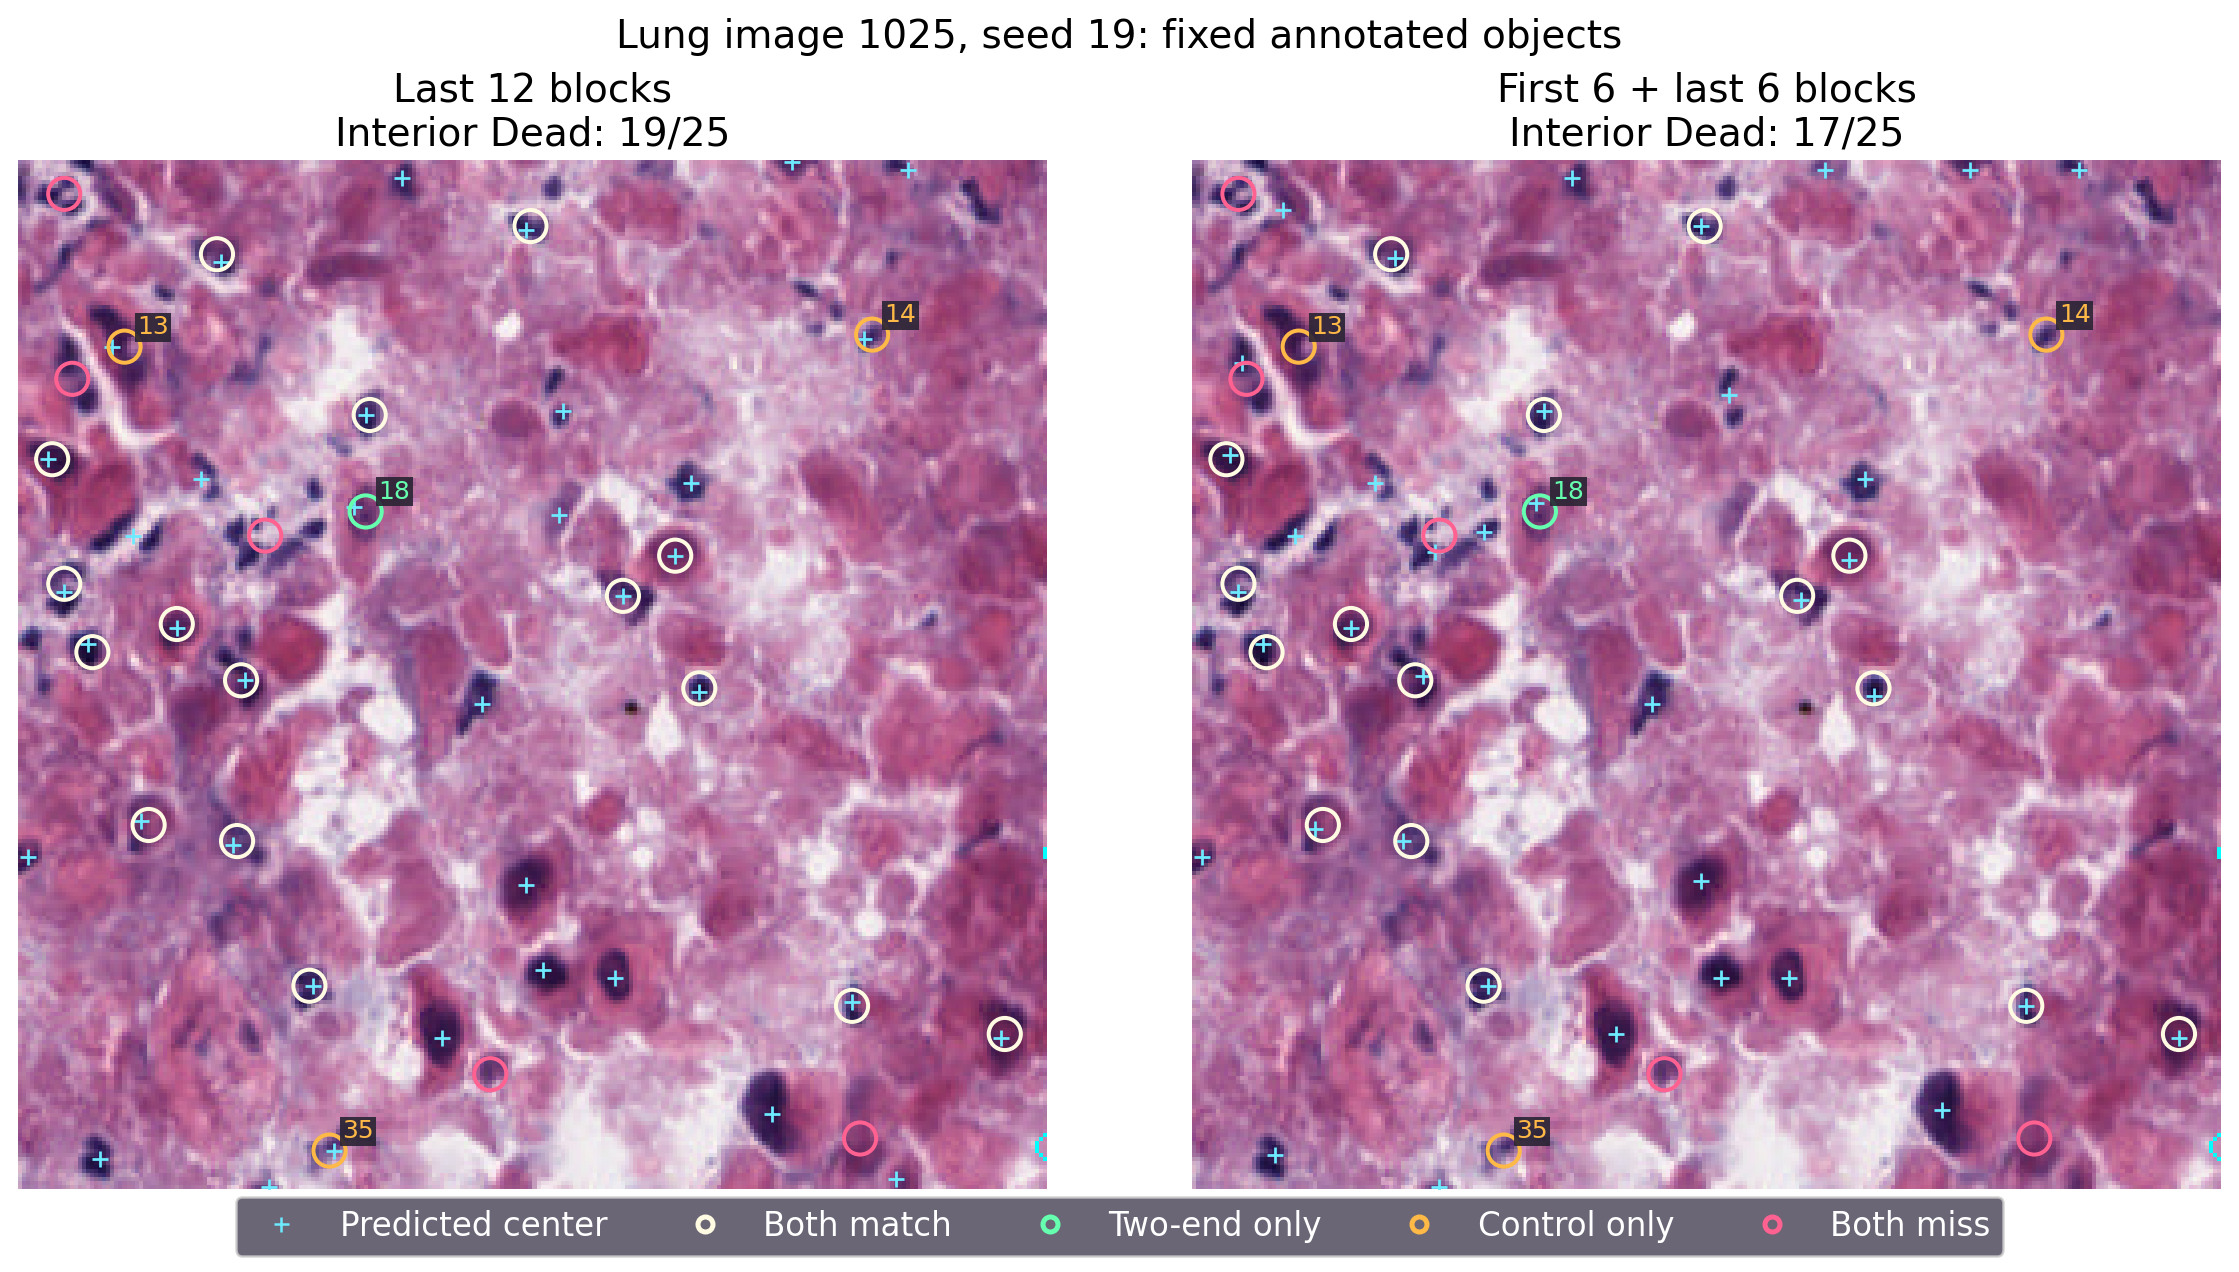
\includegraphics[width=\linewidth,height=.40\textheight,keepaspectratio]{assets/p29_image_1025_seed_19.png}
\captionof{figure}{肺组织图像 1025：新增与丢失同时发生。种子 19；左为后十二层对照，右为前六层加后六层方案。青色十字为预测中心；白、绿、橙、粉圆圈分别表示共同找到、仅新方案找到、仅对照找到和共同漏检}
\raggedright

肺组织图像 1025 从 19/25 降至 17/25。对象 18（87，86）的最近预测距离从 3.16 降至 2.24 像素，进入三像素匹配范围。对象 13（46，26）、对象 14（43，212）、对象 35（246，77）丢失匹配，距离分别从 3.00→14.56、2.24→41.77 和 1.00→18.36 像素。对象 14 面积仅 31 平方像素，视觉上也很小。实验模型在恢复一个对象的同时，失去了多个标注附近的有效输出；组织总量会掩盖这种交换。

\end{minipage}

\noindent

\begin{minipage}{\linewidth}\centering
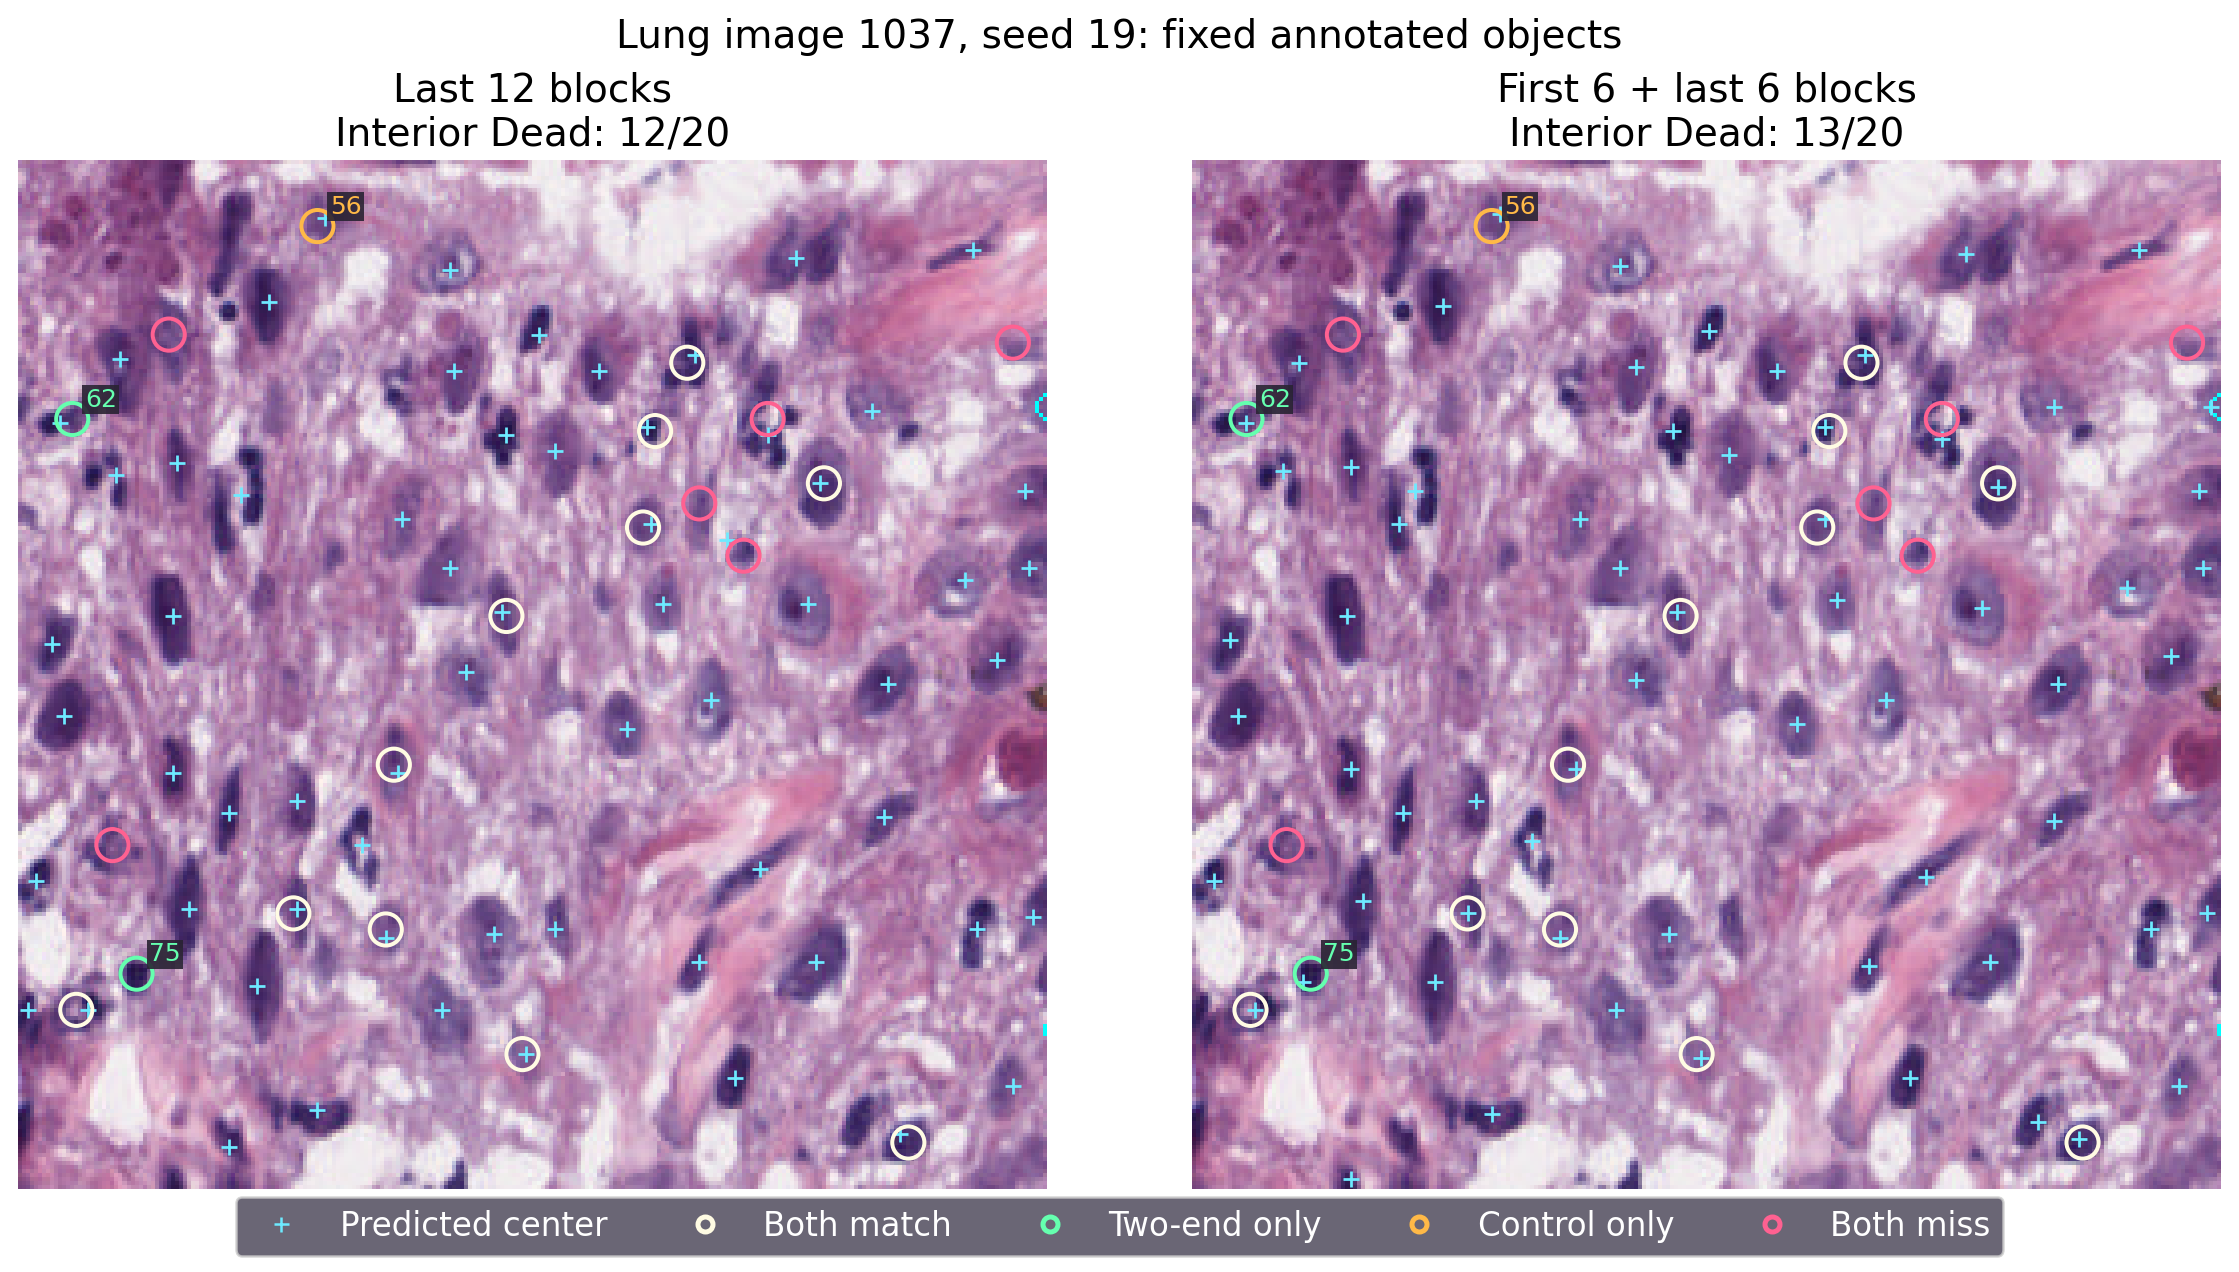
\includegraphics[width=\linewidth,height=.40\textheight,keepaspectratio]{assets/p29_image_1037_seed_19.png}
\captionof{figure}{肺组织图像 1037：小核恢复与匹配边界位移。种子 19；左为后十二层对照，右为前六层加后六层方案。青色十字为预测中心；白、绿、橙、粉圆圈分别表示共同找到、仅新方案找到、仅对照找到和共同漏检}
\raggedright

图像 1037 从 12/20 升至 13/20。对象 62（64，13）的距离从 3.16 降至 1.00 像素；面积 44 平方像素的对象 75（202，29）从 15.00 降至 2.83 像素，附近新增预测。对象 56（16，74）则因最近点从 2.83 移至 3.61 像素而失去匹配。前者表现为原来未覆盖邻域出现输出，后者表现为附近预测跨越固定匹配半径。

\end{minipage}

坐标记录确定了输出点的出现、消失和位移，原图提供染色、形态和组织环境。要把变化归因于中心分数、峰值抑制或编码器隐层，需要保存概率图或开展中间表征测量。本轮回收包含原图、标注中心、解码点和一对一匹配。

\subsubsection{种子
1：哪些改善在两个种子中一致}\label{ux79cdux5b50-1ux54eaux4e9bux6539ux5584ux5728ux4e24ux4e2aux79cdux5b50ux4e2dux4e00ux81f4}

{\def\LTcaptype{none} % do not increment counter
\begin{longtable}[]{@{}
  >{\raggedright\arraybackslash}p{(\linewidth - 12\tabcolsep) * \real{0.1111}}
  >{\raggedleft\arraybackslash}p{(\linewidth - 12\tabcolsep) * \real{0.1481}}
  >{\raggedleft\arraybackslash}p{(\linewidth - 12\tabcolsep) * \real{0.1481}}
  >{\raggedleft\arraybackslash}p{(\linewidth - 12\tabcolsep) * \real{0.1481}}
  >{\raggedleft\arraybackslash}p{(\linewidth - 12\tabcolsep) * \real{0.1481}}
  >{\raggedleft\arraybackslash}p{(\linewidth - 12\tabcolsep) * \real{0.1481}}
  >{\raggedleft\arraybackslash}p{(\linewidth - 12\tabcolsep) * \real{0.1481}}@{}}
\toprule\noalign{}
\begin{minipage}[b]{\linewidth}\raggedright
种子 1 更新范围
\end{minipage} & \begin{minipage}[b]{\linewidth}\raggedleft
内部死亡细胞核
\end{minipage} & \begin{minipage}[b]{\linewidth}\raggedleft
小型死亡细胞核
\end{minipage} & \begin{minipage}[b]{\linewidth}\raggedleft
全部匹配
\end{minipage} & \begin{minipage}[b]{\linewidth}\raggedleft
总召回
\end{minipage} & \begin{minipage}[b]{\linewidth}\raggedleft
精度
\end{minipage} & \begin{minipage}[b]{\linewidth}\raggedleft
未匹配预测
\end{minipage} \\
\midrule\noalign{}
\endhead
\bottomrule\noalign{}
\endlastfoot
最后十二层 & 67/145 & 7/32 & 7,329/12,250 & 59.83\% & 69.25\% & 3,255 \\
前六层＋后六层 & 80/145 & 11/32 & 7,494/12,250 & 61.18\% & 70.14\% &
3,191 \\
\end{longtable}
}

种子 1 多找到 13 个目标核，内部死亡细胞核召回增加 8.9655
个百分点，原固定重采样的 95\%
区间为［+3.1250，+20.4082］个百分点。实验模型多输出 101 个点、多匹配 165
个核。两个种子的总体召回、精度和小型死亡细胞核覆盖均改善，训练集覆盖均下降；最终死亡细胞核召回和精度均未达到
0.60/0.75，两种子均未满足原定的完整条件。两种子配对变化的描述性均值为死亡细胞核召回
+10.0 个百分点、总体召回 +1.83 个百分点、精度 +1.06
个百分点。两个种子使用相同图像，均值汇总重复训练结果，两次训练使用同样的
522 张开发评估图像。

种子 1 有五张图像增加、一张减少、五张不变。肺组织贡献 +6，宫颈 +5，结肠
+1，食管 +1。肺组织图像 1038 在种子 19/1 中分别增加 5/4 个；宫颈图像
1756 增加 2/5 个。结肠图像 1482 则分别为 13/49→13/49 和
11/49→10/49，仍遗漏 36/39 个目标核。肺组织图像 1025
在两个种子中的净变化为
−2/+2。总体改善同方向，贡献图像与具体对象却有差异。种子 1
逐一去掉一张包含死亡细胞核的图像后，改善仍为 +6.15～+14.58
个百分点；种子 19 为 +8.03～+16.67 个百分点。

训练集总体召回从 97.80\% 降至 95.43\%，内部死亡细胞核匹配从 624/656 降至
606/656。记录的训练时间为 4.0143/6.7220 小时，检查点写入时间为
238.77/2,116.75 秒，实验模型完成训练和评估的应用总耗时为 10.1409
小时。种子 1 实验模型经历了长时间 Lustre
延迟，这些耗时包含等待，用于记录实际资源成本；种子 19 的 21.24\%
训练时间增加更适合描述本轮更新范围的常规成本差异。两种子的训练峰值已分配显存均约为
4.05/4.84 GiB。

\subsubsection{固定对象：重复恢复、重复丢失与相互抵消}\label{ux56faux5b9aux5bf9ux8c61ux91cdux590dux6062ux590dux91cdux590dux4e22ux5931ux4e0eux76f8ux4e92ux62b5ux6d88}

种子 1 的八张固定样例共同找到 29 个、新增 7 个、丢失 3 个、共同漏检 14
个，53 个目标对象净增加 4 个；种子 19 分别为 30、6、4、13，净增加 2
个。以下分析沿用相同标注编号和原始坐标。

\noindent

\begin{minipage}{\linewidth}\centering
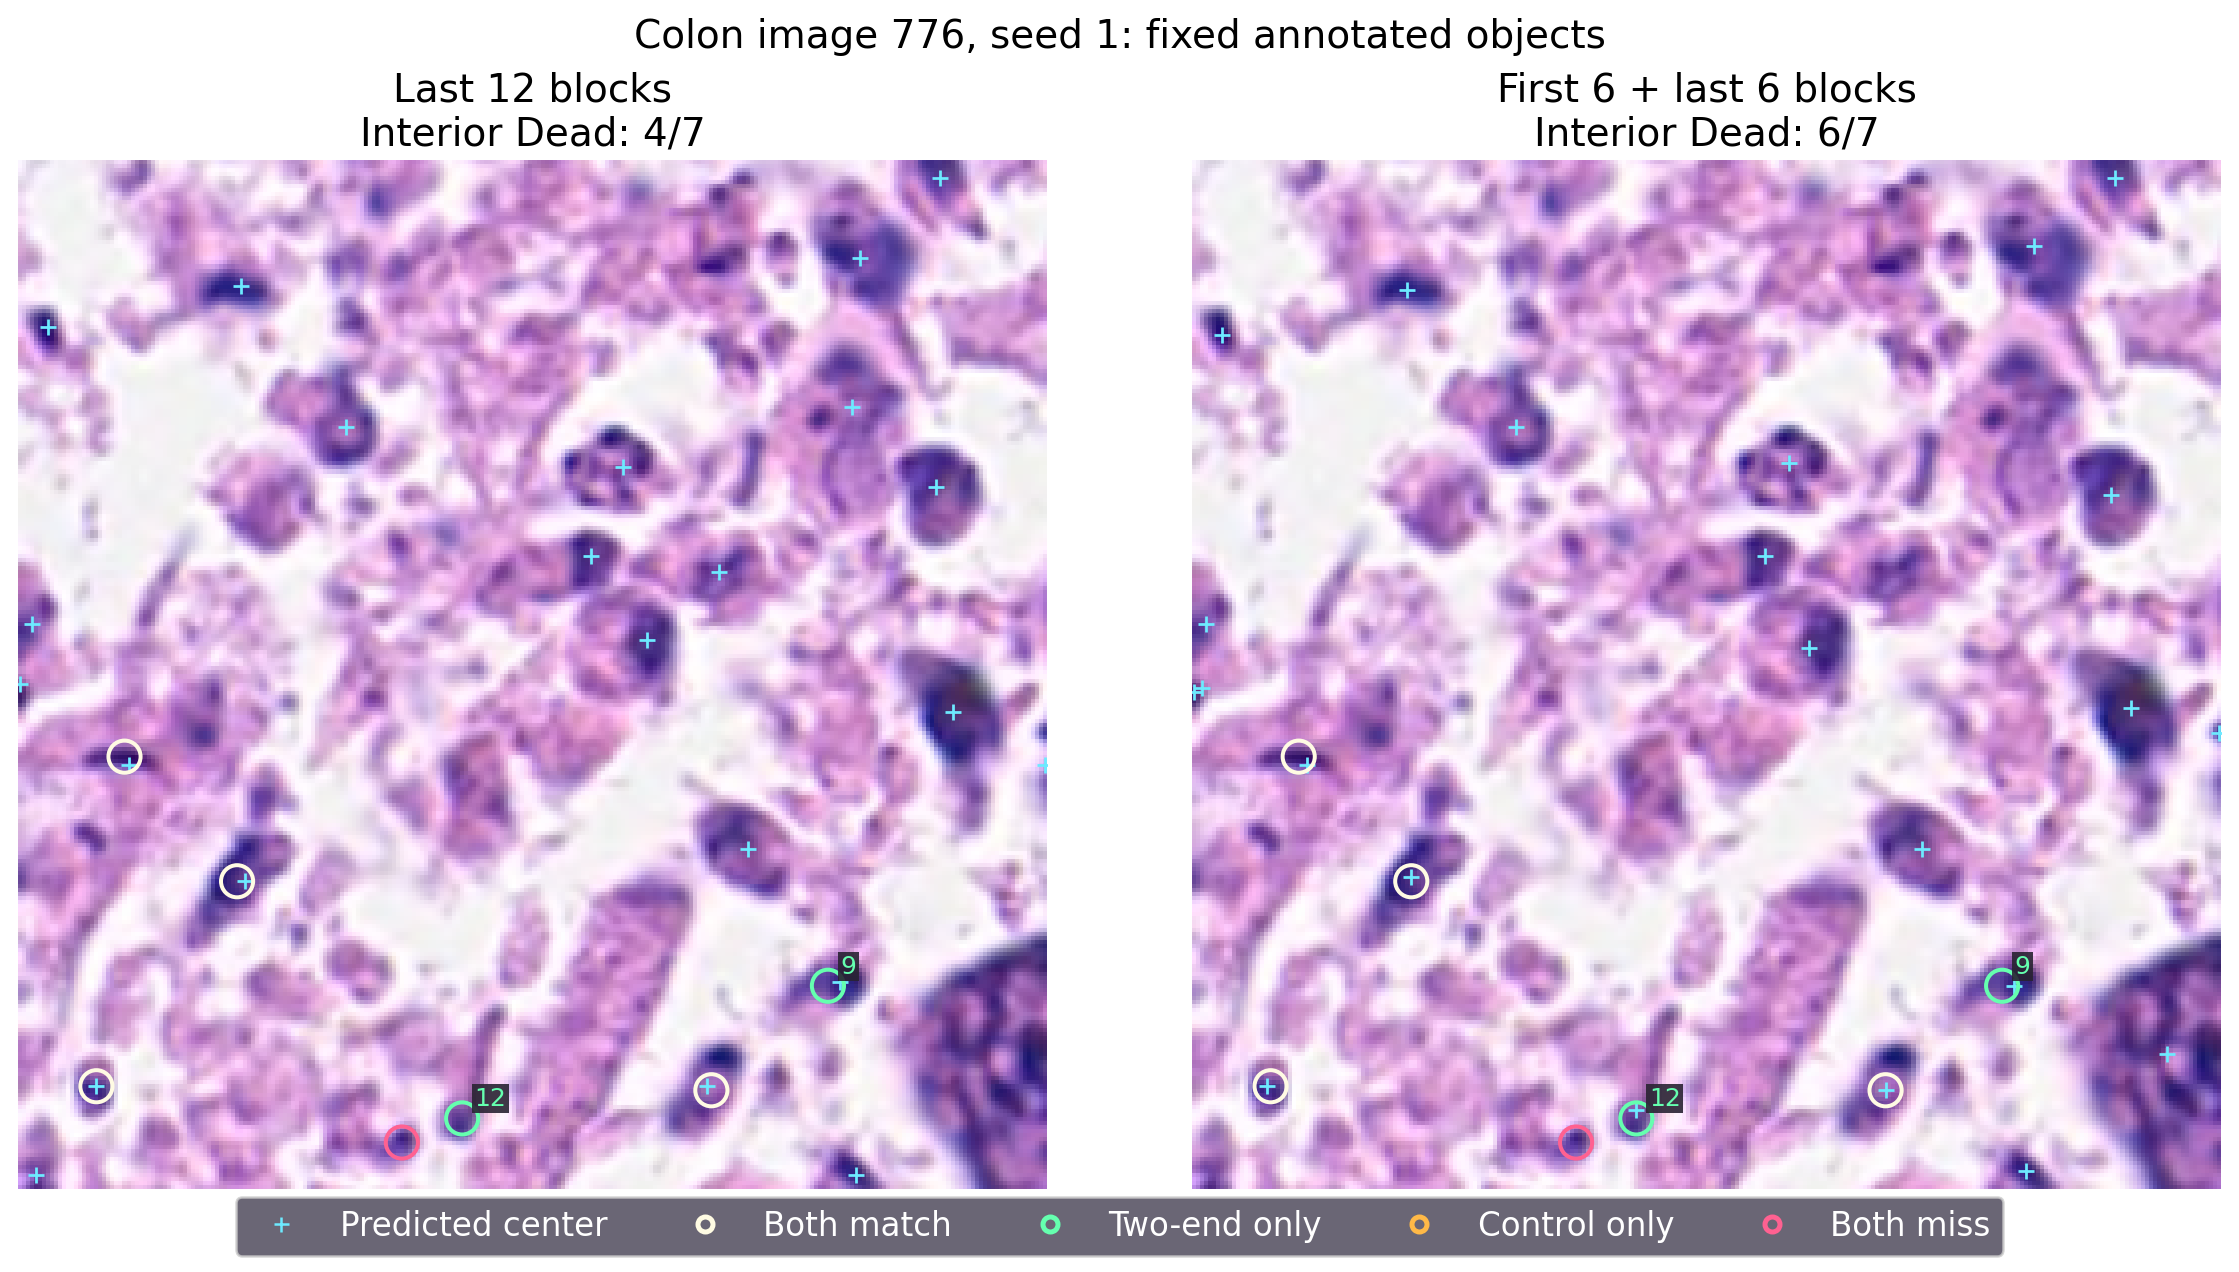
\includegraphics[width=\linewidth,height=.40\textheight,keepaspectratio]{assets/p29_image_776_seed_1.png}
\captionof{figure}{种子 1 的结肠图像 776。种子 1；左为后十二层对照，右为前六层加后六层方案。青色十字为预测中心；白、绿、橙、粉圆圈分别表示共同找到、仅新方案找到、仅对照找到和共同漏检}
\raggedright

结肠图像 776 从 4/7 增至 6/7。对象 12 位于（238，110），面积为 104 平方像素，在两个种子中均被找回：最近点距离在种子 19 为 80.66→1.00，种子 1 为 61.52→2.00 像素。这是在同一个标注上重复观察到的恢复。种子 1 还找回对象 9（205，201），面积 191 平方像素，距离从 3.16 降至 3.00 像素；种子 19 则找回下方组织带中的对象 10 和 11。相似的图像总改善可以来自不同细胞核。

\end{minipage}

\noindent

\begin{minipage}{\linewidth}\centering
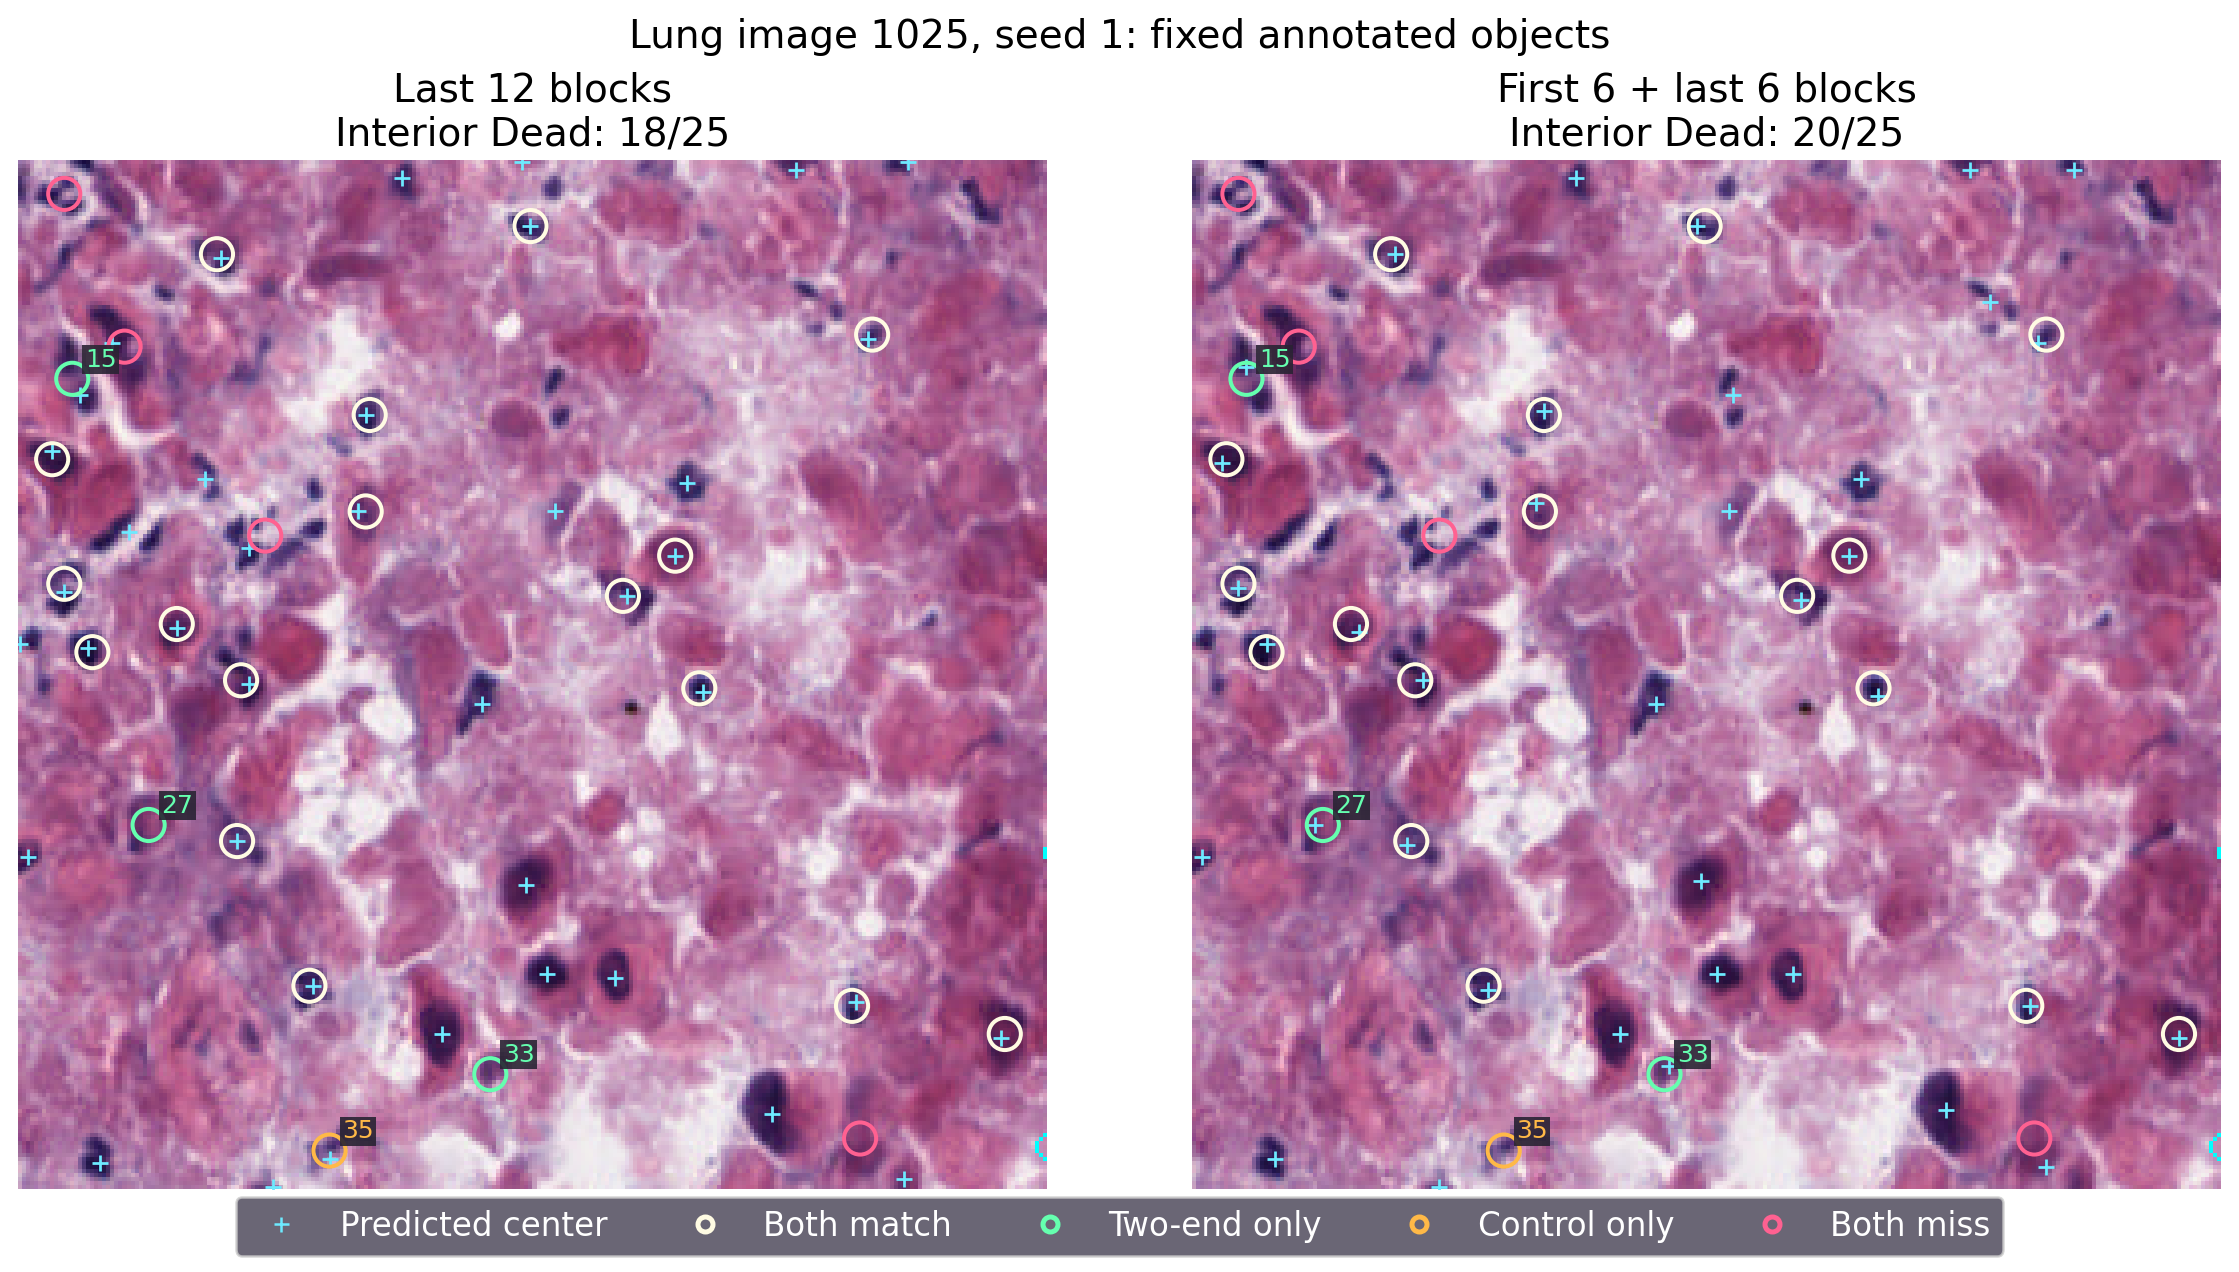
\includegraphics[width=\linewidth,height=.40\textheight,keepaspectratio]{assets/p29_image_1025_seed_1.png}
\captionof{figure}{种子 1 的肺组织图像 1025。种子 1；左为后十二层对照，右为前六层加后六层方案。青色十字为预测中心；白、绿、橙、粉圆圈分别表示共同找到、仅新方案找到、仅对照找到和共同漏检}
\raggedright

图像 1025 从 18/25 增至 20/25。对象 15（54，13）、27（165，32）、33（227，117）新增匹配，距离分别为 4.47→3.00、22.36→2.00、15.62→2.24 像素。对象 33 面积 52 平方像素，属于预定义的小核组。对象 35（246，77）面积 68 平方像素，在两个种子中均丢失：种子 19 为 1.00→18.36，种子 1 为 2.00→18.36 像素。重复出现的局部丢失与肺组织总量的改善同时存在。

\end{minipage}

\noindent

\begin{minipage}{\linewidth}\centering
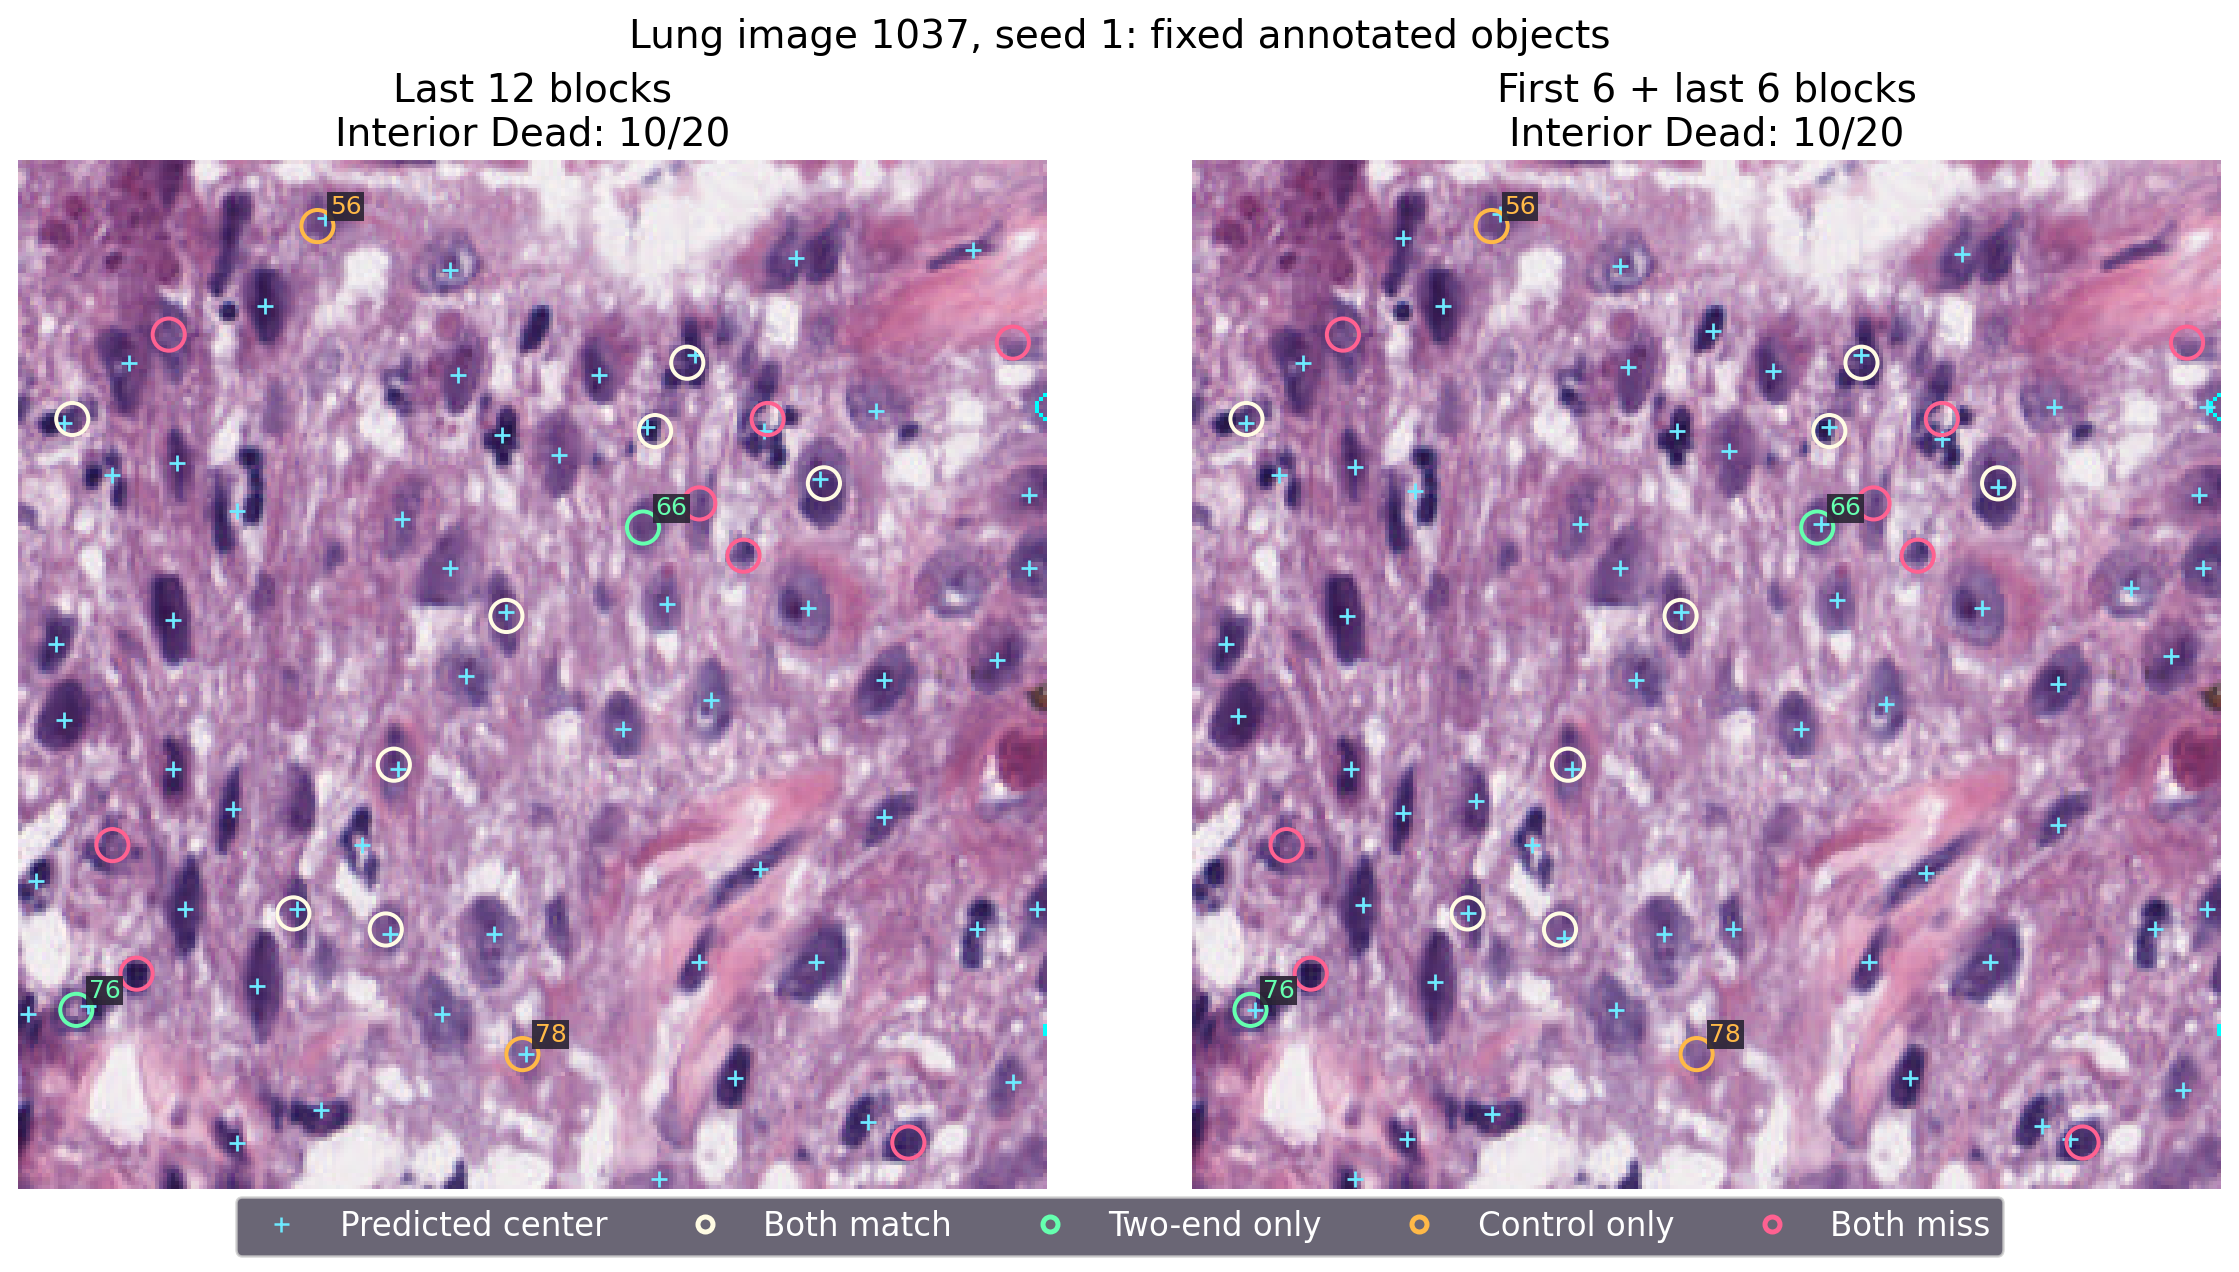
\includegraphics[width=\linewidth,height=.40\textheight,keepaspectratio]{assets/p29_image_1037_seed_1.png}
\captionof{figure}{种子 1 的肺组织图像 1037。种子 1；左为后十二层对照，右为前六层加后六层方案。青色十字为预测中心；白、绿、橙、粉圆圈分别表示共同找到、仅新方案找到、仅对照找到和共同漏检}
\raggedright

图像 1037 保持 10/20，但内部发生两个新增和两个丢失。对象 66（91，155）、76（211，14）距离为 19.92→1.41 和 3.16→1.00；对象 56（16，74）、78（222，125）距离为 2.83→3.61 和 1.00→22.83 像素。对象 56 在两个种子中跨越了完全相同的匹配边界。因此，图像匹配数不变也可能包含重复的定位丢失，以及其他核的补偿恢复。全部逐核距离、预测中心和一对一分配均保存在坐标 JSON 与 CSV 中。

\end{minipage}

\subsection{P30：训练中间十二层}\label{p30ux8badux7ec3ux4e2dux95f4ux5341ux4e8cux5c42}

P30 将可训练范围从第 12--23 层改为第 6--17
层（层号从零开始），编码器及检测头参数量、学习率和训练计划保持一致。数组
55746187 四项均正常完成，包含连续 130
轮训练和最后检查点开发评估；调度总耗时为 17.4389 GPU 小时。

{\def\LTcaptype{none} % do not increment counter
\begin{longtable}[]{@{}
  >{\raggedright\arraybackslash}p{(\linewidth - 12\tabcolsep) * \real{0.1111}}
  >{\raggedleft\arraybackslash}p{(\linewidth - 12\tabcolsep) * \real{0.1481}}
  >{\raggedleft\arraybackslash}p{(\linewidth - 12\tabcolsep) * \real{0.1481}}
  >{\raggedleft\arraybackslash}p{(\linewidth - 12\tabcolsep) * \real{0.1481}}
  >{\raggedleft\arraybackslash}p{(\linewidth - 12\tabcolsep) * \real{0.1481}}
  >{\raggedleft\arraybackslash}p{(\linewidth - 12\tabcolsep) * \real{0.1481}}
  >{\raggedleft\arraybackslash}p{(\linewidth - 12\tabcolsep) * \real{0.1481}}@{}}
\toprule\noalign{}
\begin{minipage}[b]{\linewidth}\raggedright
运行
\end{minipage} & \begin{minipage}[b]{\linewidth}\raggedleft
内部死亡细胞核
\end{minipage} & \begin{minipage}[b]{\linewidth}\raggedleft
小型死亡细胞核
\end{minipage} & \begin{minipage}[b]{\linewidth}\raggedleft
总体匹配
\end{minipage} & \begin{minipage}[b]{\linewidth}\raggedleft
预测点
\end{minipage} & \begin{minipage}[b]{\linewidth}\raggedleft
召回率
\end{minipage} & \begin{minipage}[b]{\linewidth}\raggedleft
精确率
\end{minipage} \\
\midrule\noalign{}
\endhead
\bottomrule\noalign{}
\endlastfoot
种子 19，最后十二层 & 71／145 & 9／32 & 7,246 & 10,539 & 59.151\% &
68.754\% \\
种子 19，中间十二层 & 78／145 & 14／32 & 7,894 & 10,972 & 64.441\% &
71.947\% \\
种子 1，最后十二层 & 64／145 & 8／32 & 7,338 & 10,647 & 59.902\% &
68.921\% \\
种子 1，中间十二层 & 79／145 & 13／32 & 7,854 & 10,909 & 64.114\% &
71.996\% \\
\end{longtable}
}

新方案增加 433／262 个预测点，同时增加 648／516
个正确匹配，因此额外点减少 215／254 个。总体召回提高 5.2898／4.2122
个百分点，精确率提高 3.1926／3.0748
个百分点。两个种子的小型死亡细胞核匹配均增加五个。内部死亡细胞核召回提高
4.8276／10.3448 个百分点，原 95\% 成对区间为 {[}−0.9091,+9.6552{]} 和
{[}+1.8987,+18.3673{]} 个百分点。

原定条件要求死亡细胞核检出率至少 60\%、匹配精度至少
75\%，还要求相对对照的改善达到规定水平。两次实验的死亡细胞核检出率为
53.79\%／54.48\%，匹配精度为
71.95\%／72.00\%；这一固定中间十二层方案按原规则完成收尾。

\subsubsection{P30
的组织分布、敏感性与计算成本}\label{p30-ux7684ux7ec4ux7ec7ux5206ux5e03ux654fux611fux6027ux4e0eux8ba1ux7b97ux6210ux672c}

肺组织贡献 +5／+9，结肠贡献 +3／+6，宫颈在两个种子中均减少一个。肺组织
1037 增加四／六个，1038 增加二／四个，结肠 1482 增加三／五个；肺组织
1025 在两个种子中均减少一个。结肠 1482 最终找到 17／49 和 16／49
个目标，仍有 32／33
个未覆盖。其净收益减少了集中图像中的漏检，同时保留了清晰的后续改善空间。

种子 19 有三张目标图像净增、两张净减、六张不变；种子 1
有五张净增、两张净减、四张不变。逐次移除一张包含目标细胞核的图像进行描述性敏感性计算，召回收益范围分别为
2.40--6.67 和 7.20--13.33
个百分点。收益符号在任一单图移除后均保留；原自助区间继续刻画完整固定图像集合的重抽样不确定性。

训练总体召回变化 97.85\%→97.10\% 和 98.05\%→97.12\%。种子 19
的训练过程耗时为 14,457.50 与 15,957.59 秒；种子 1 为 14,509.86 与
15,957.90 秒，增加约 10.4\% 和 10.0\%。峰值训练显存由约 4.05 增至 4.44
GiB。中间层适配在相同参数量下，以适中的实测成本带来了较广泛的开发集检测收益；冻结层前后的梯度路径变化仍会影响计算。

\subsubsection{P30
固定对象：新增、丢失和种子变化}\label{p30-ux56faux5b9aux5bf9ux8c61ux65b0ux589eux4e22ux5931ux548cux79cdux5b50ux53d8ux5316}

八张预先固定的开发样例包含 53 个内部死亡细胞核。种子 19 共同找到 29
个、新增八个、丢失五个、两组均漏检十一；种子 1 对应为
26、十一、五、十一，净增
+3／+6。绿色环表示仅新方案找到，橙色环表示仅对照找到，白色表示共同找到，粉色表示共同漏检，青色十字为模型预测点。对象编号、行列坐标与匹配记录均随报告保存。

\noindent

\begin{minipage}{\linewidth}\centering
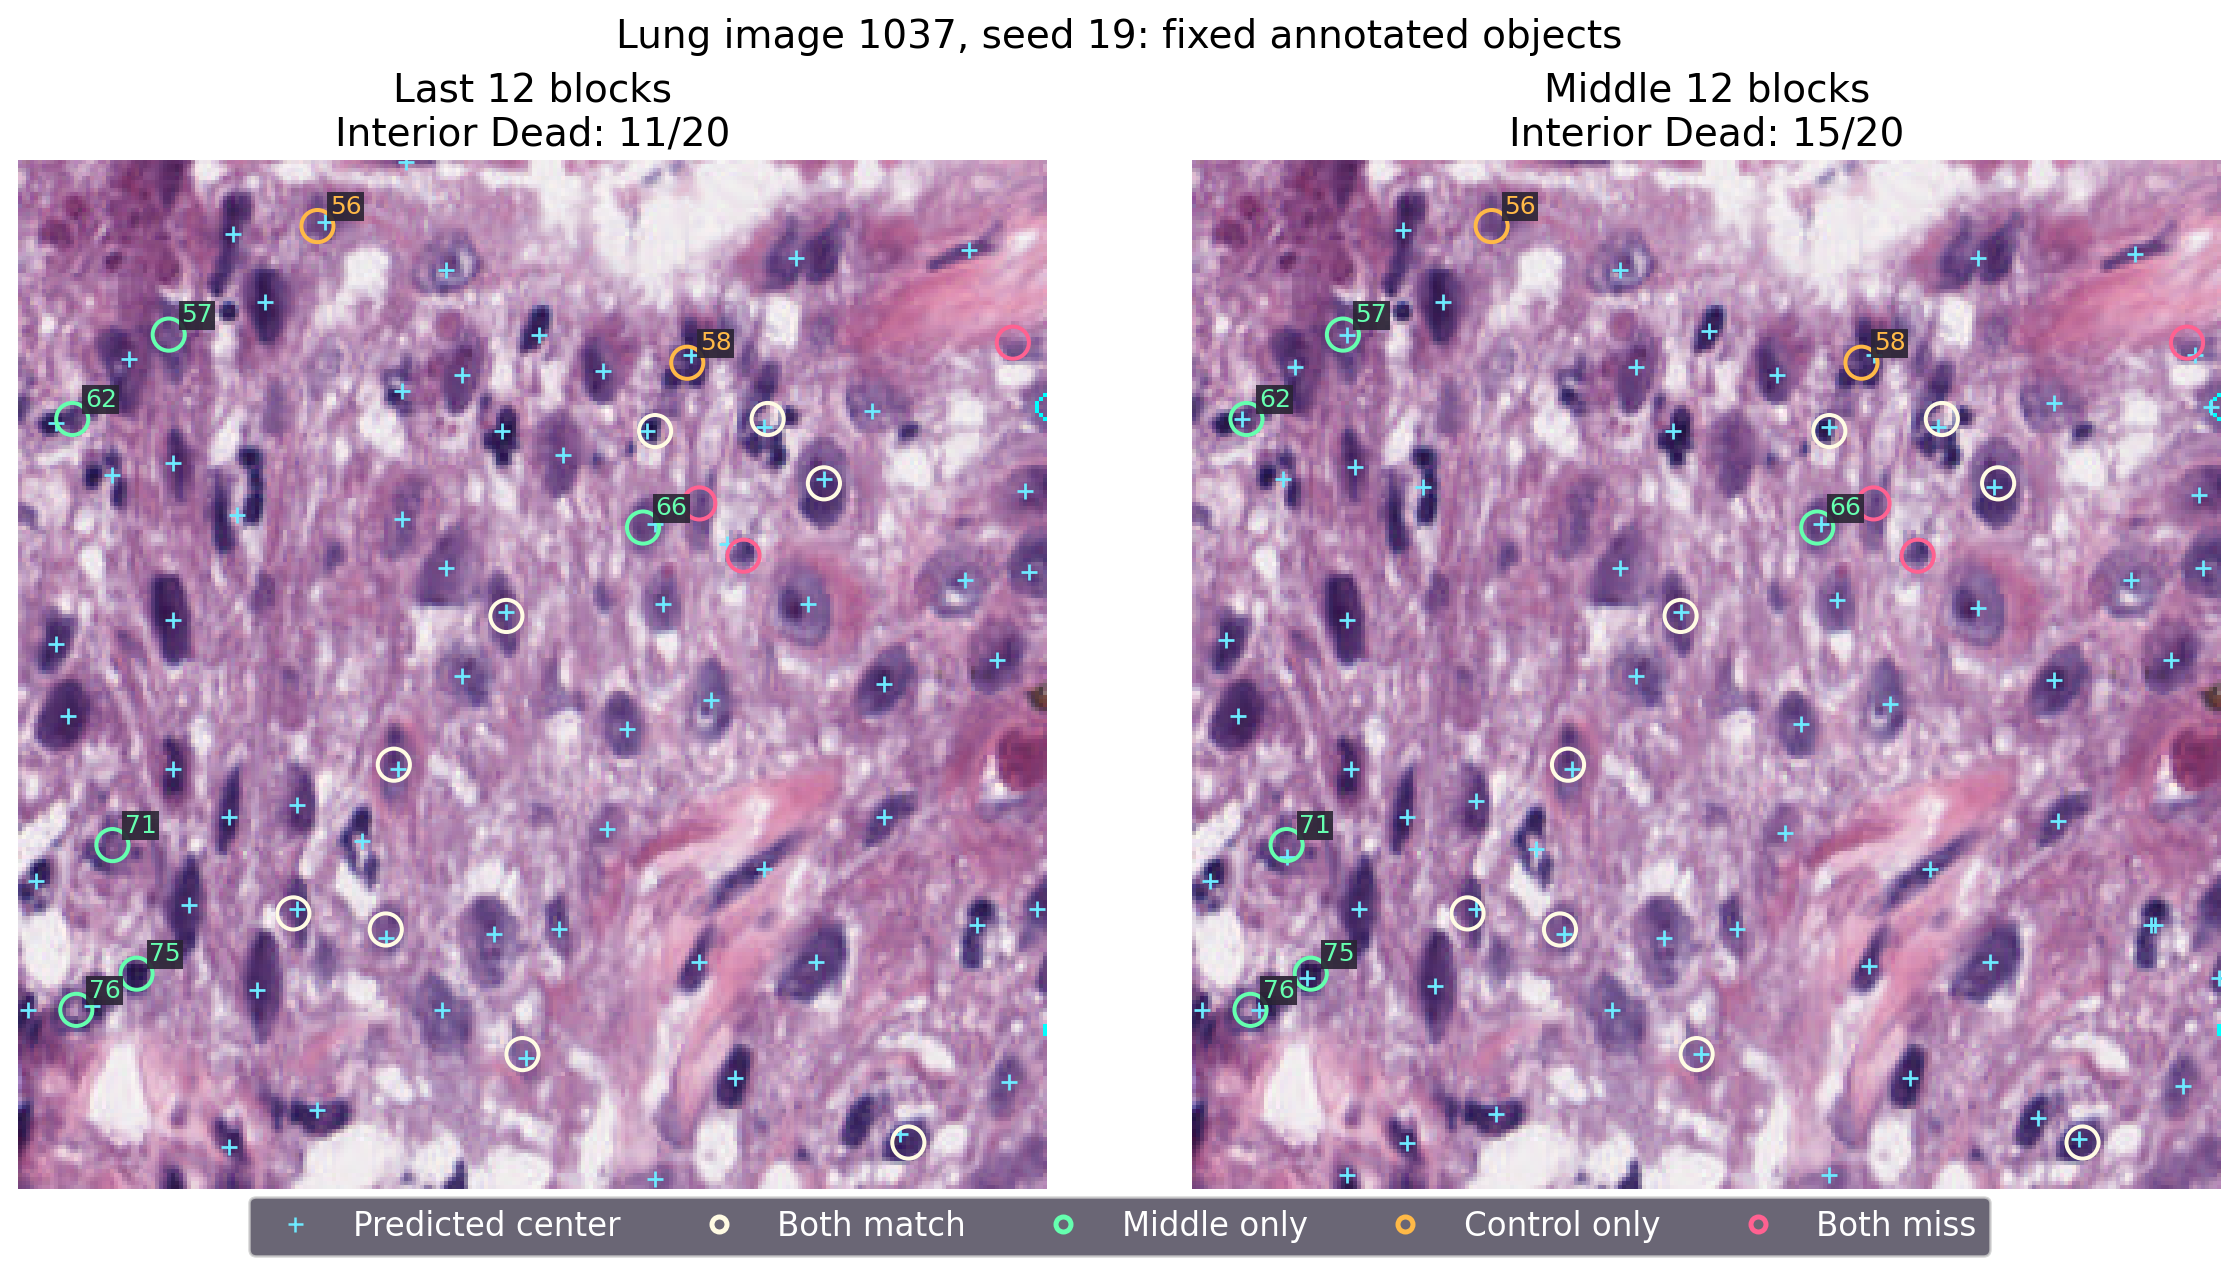
\includegraphics[width=\linewidth,height=.40\textheight,keepaspectratio]{assets/p30_image_1037_seed_19.png}
\captionof{figure}{P30，肺组织图像 1037，种子 19：六个新增与两个丢失。种子 19；左为后十二层对照，右为中间十二层方案。青色十字为预测中心；白、绿、橙、粉圆圈分别表示共同找到、仅新方案找到、仅对照找到和共同漏检}
\raggedright

该图由 11／20 提高至 15／20。小核 75 位于 (202,29)，面积 44 平方像素，距离变化 13.60→1.41；该左下标注位置在多种此前方案中也被恢复。对象 57 位于 (43,37)，是一枚邻近较深色组织的浅色圆核，距离由 11.66 降至 1.00。对象 62、66、71、76 也新增匹配。对象 56 位于 (16,74)，由 2.24 增至 22.02；对象 58 位于 (50,166)，由 2.24 增至 3.61。前者附近留下较大预测空隙，后者通过位置变化跨过匹配边界。

\end{minipage}

\noindent

\begin{minipage}{\linewidth}\centering
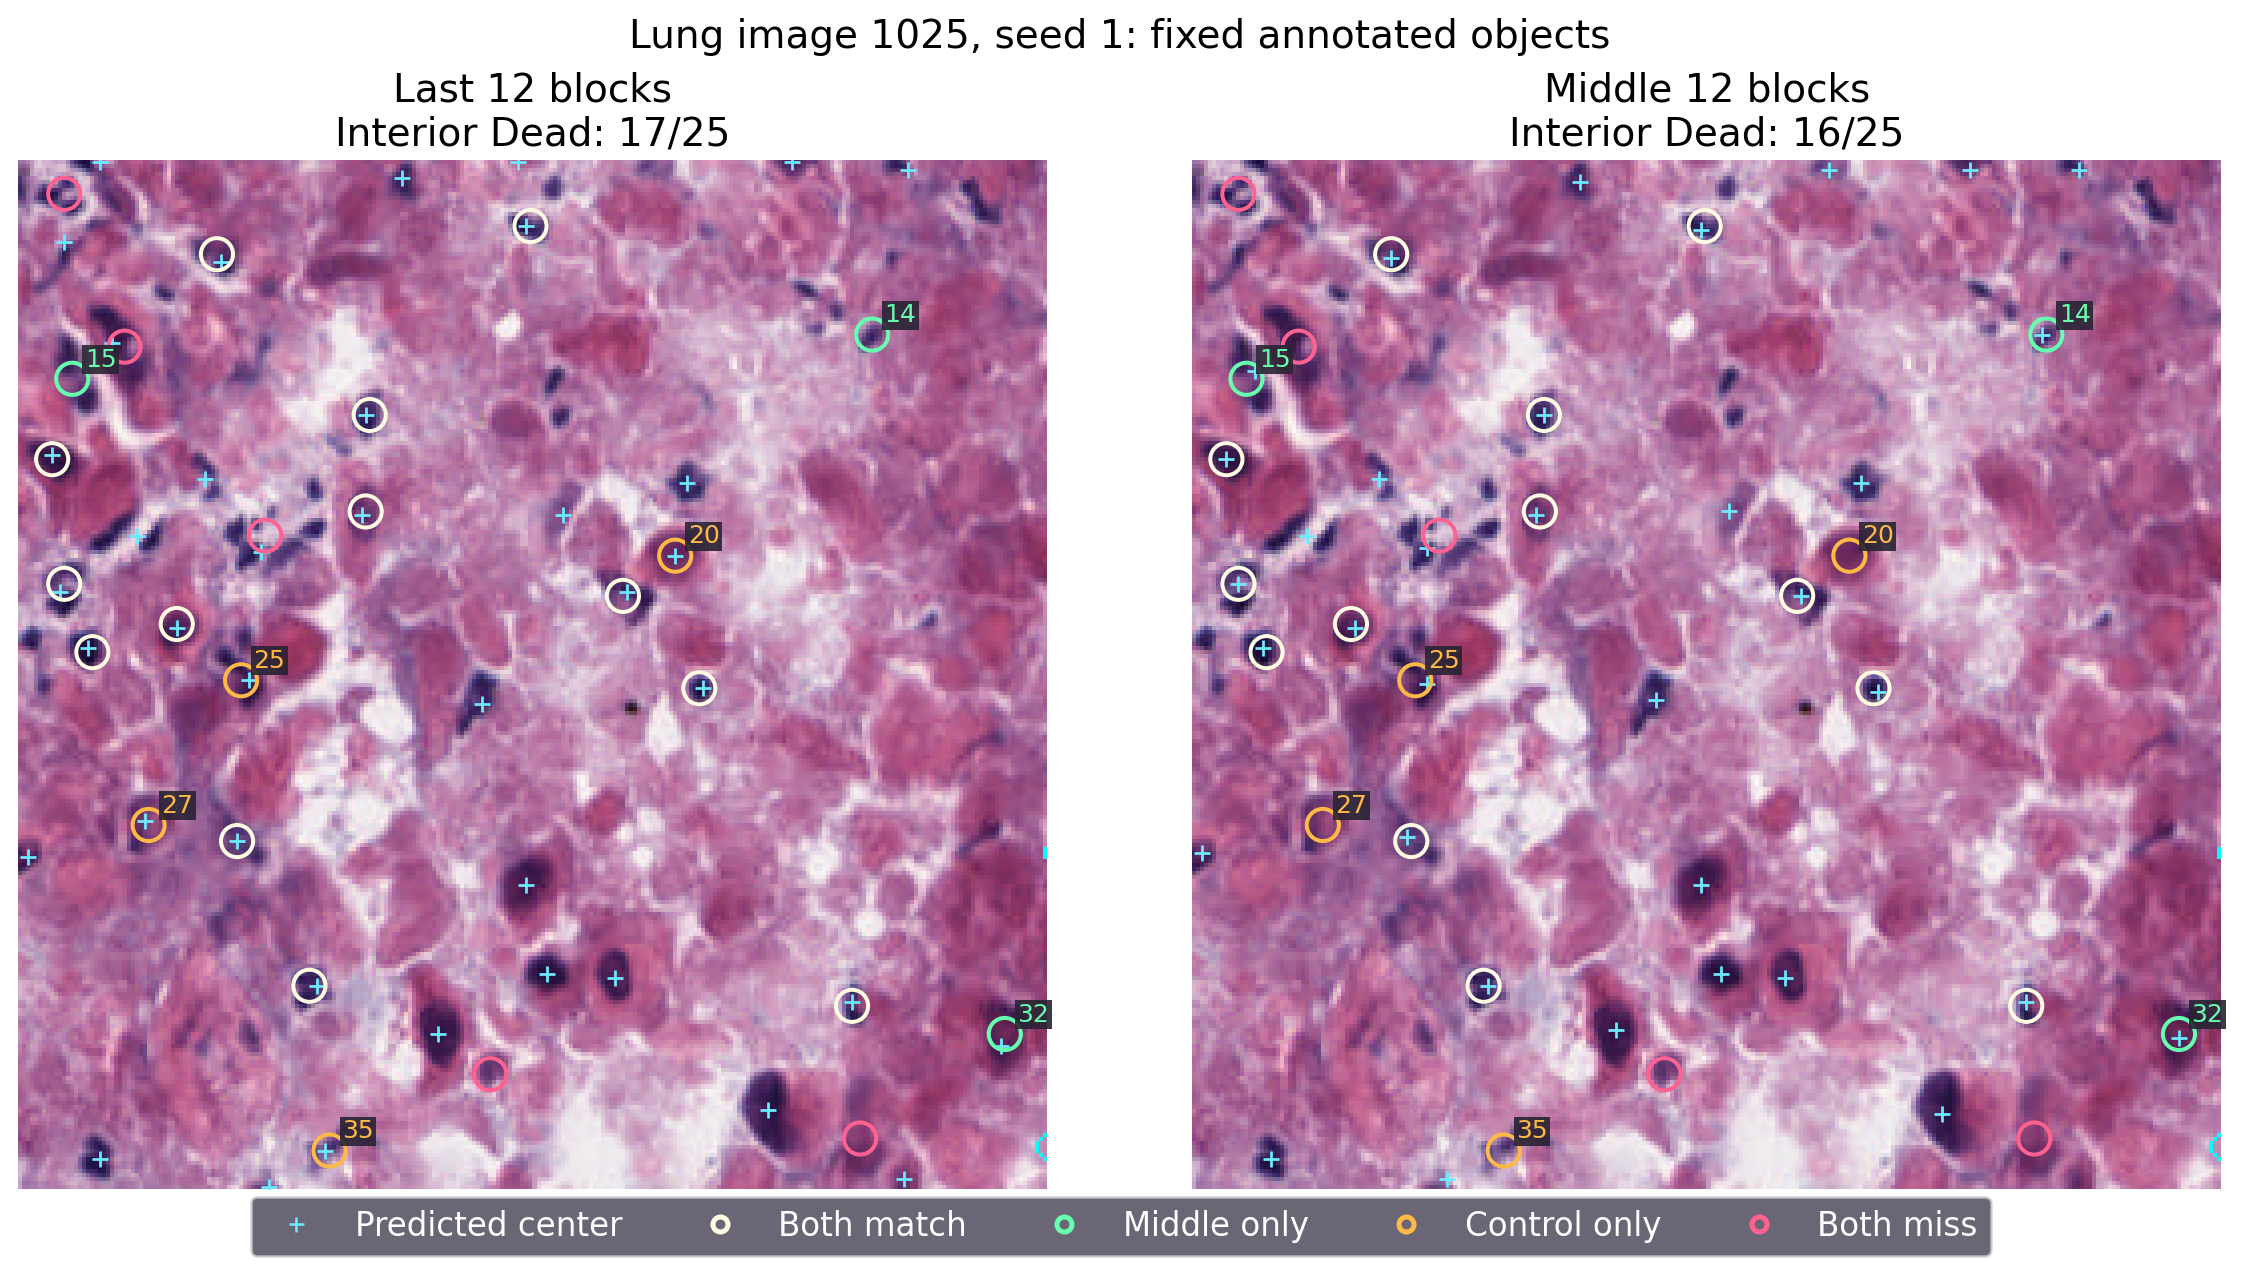
\includegraphics[width=\linewidth,height=.40\textheight,keepaspectratio]{assets/p30_image_1025_seed_1.png}
\captionof{figure}{P30，肺组织图像 1025，种子 1：恢复小核，同时丢失四个已有匹配。种子 1；左为后十二层对照，右为中间十二层方案。青色十字为预测中心；白、绿、橙、粉圆圈分别表示共同找到、仅新方案找到、仅对照找到和共同漏检}
\raggedright

该图由 17／25 降至 16／25，具体为三个新增、四个丢失。小核 14 位于 (43,212)，面积 31 平方像素，最近距离由 41.98 降至 1.00。对象 15 (54,13) 由 13.45 降至 2.83，对象 32 (217,245) 由 3.16 移至 1.00。对象 20 (98,163)、27 (165,32)、35 (246,77) 丢失附近预测，最近距离分别增至 15.62、21.21、15.65。对象 25 (129,55) 由 2.00 移至 3.16，刚好跨出匹配范围。相同小核 14 在种子 19 中反向变化，2.00→41.98。该对象具体展示了训练随机性，而这张图的总体净减在两个种子中重复出现。

\end{minipage}

\noindent

\begin{minipage}{\linewidth}\centering
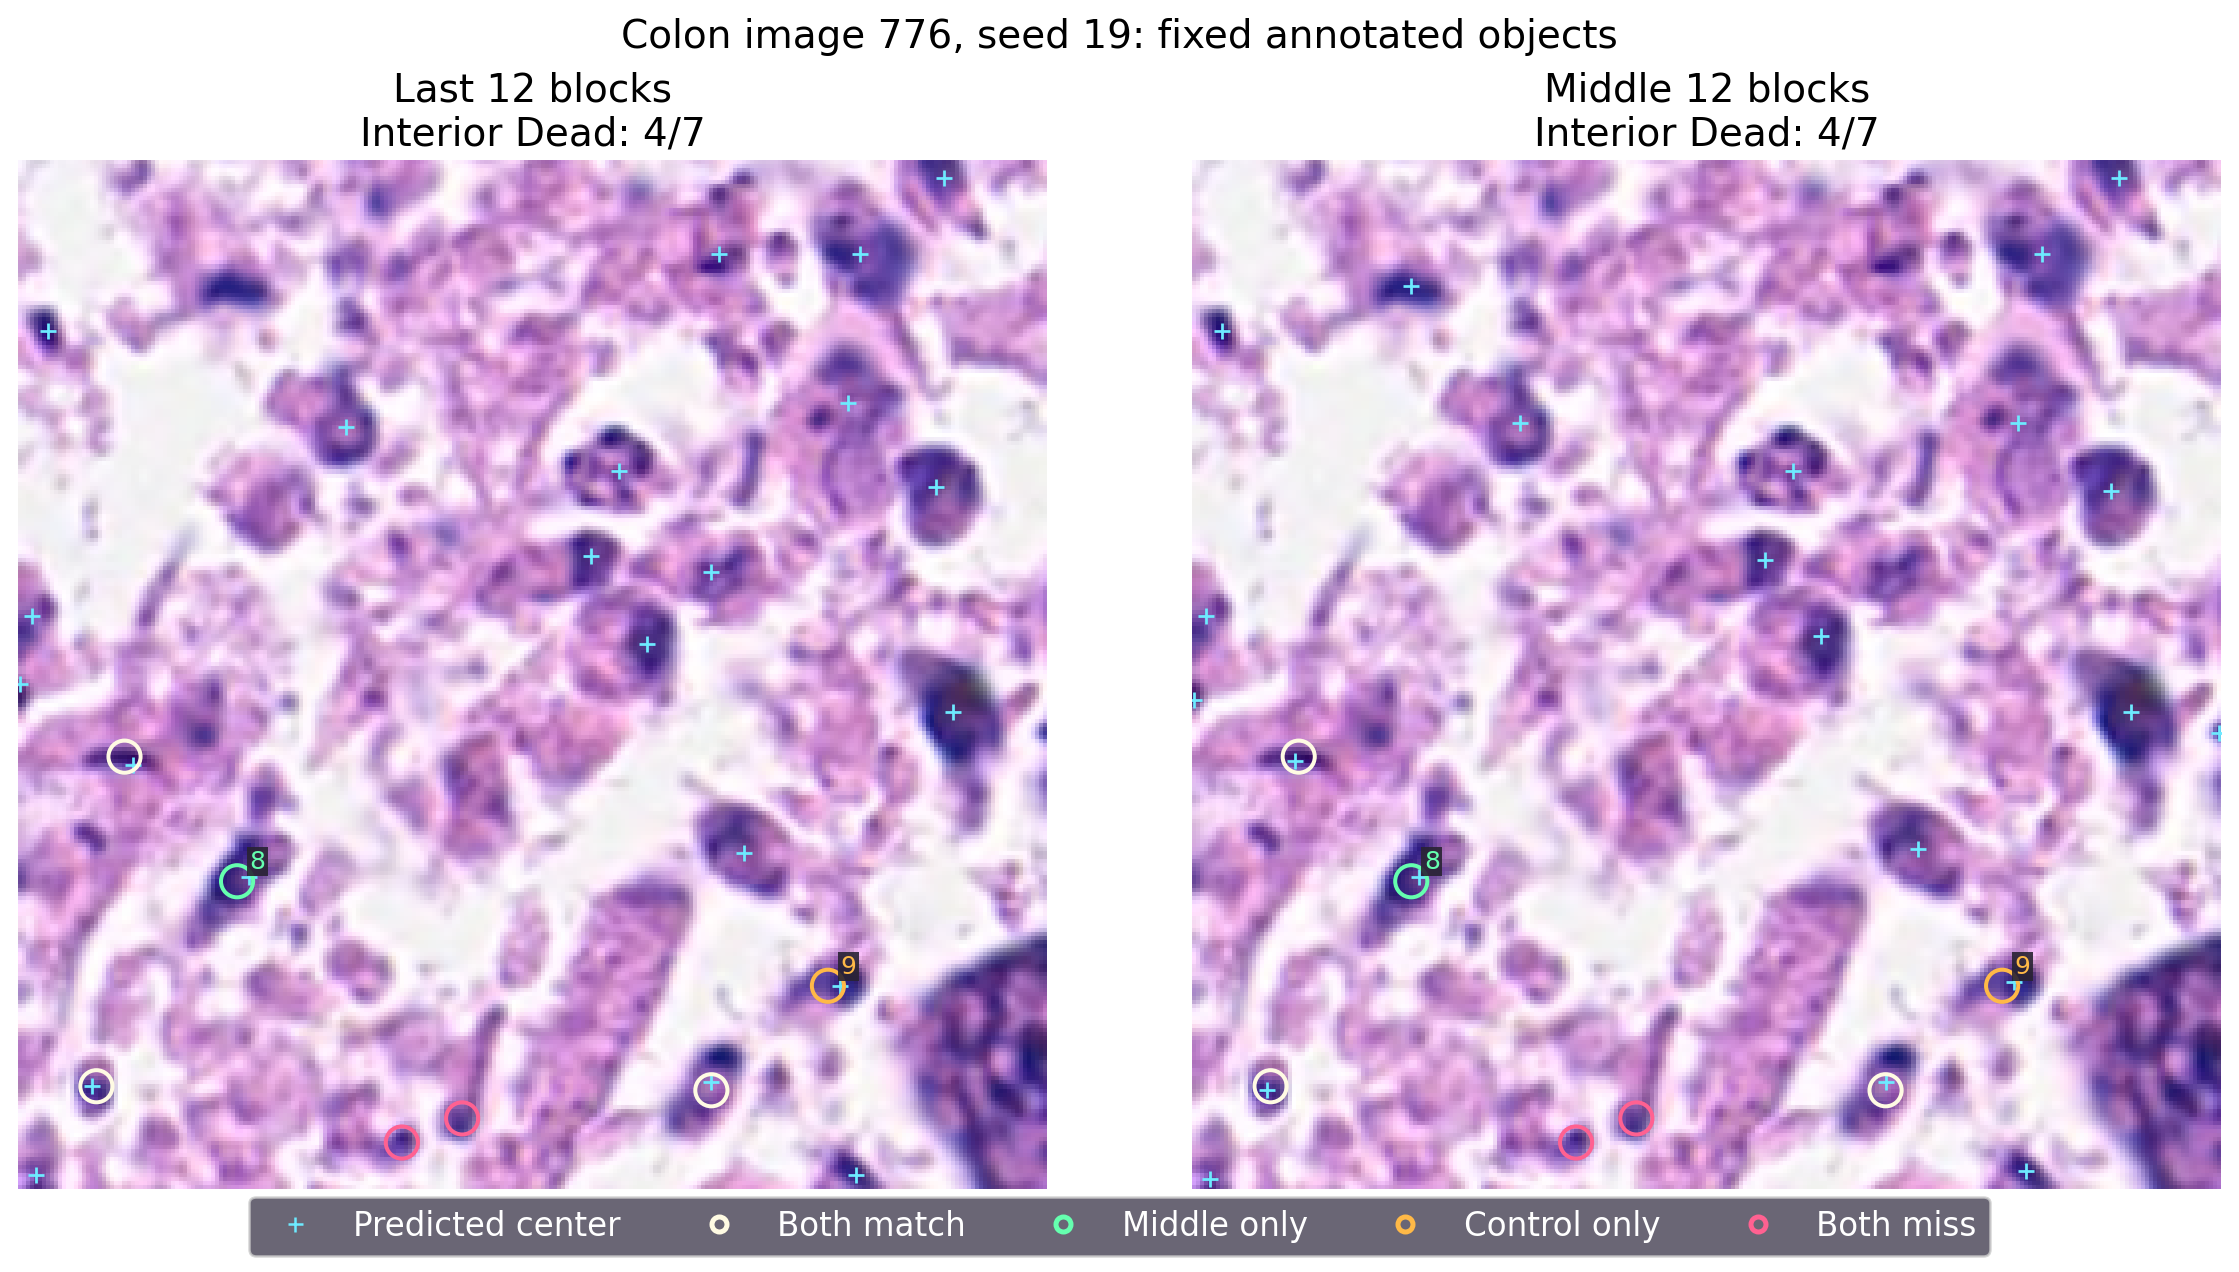
\includegraphics[width=\linewidth,height=.40\textheight,keepaspectratio]{assets/p30_image_776_seed_19.png}
\captionof{figure}{P30，结肠组织图像 776，种子 19：相同计数下的对象交换。种子 19；左为后十二层对照，右为中间十二层方案。青色十字为预测中心；白、绿、橙、粉圆圈分别表示共同找到、仅新方案找到、仅对照找到和共同漏检}
\raggedright

该图保持 4／7，但对象 8 (179,54) 新增，3.16→2.24；对象 9 (205,201) 丢失，3.00→3.16。两者都靠近匹配边界。种子 1 恢复对象 9，整图升至 5／7。相同的种子 19 计数因此包含了不同对象之间的交换。保存的坐标直接刻画预测点出现、消失和移动；后续机制研究可通过完整概率图和中间特征统计进一步测量中心分数及峰值选择。

\end{minipage}

\subsection{P31：在检测头中加入分组归一化}\label{p31ux5728ux68c0ux6d4bux5934ux4e2dux52a0ux5165ux5206ux7ec4ux5f52ux4e00ux5316}

P31
将八个分组归一化模块加入细胞核中心检测头；这种方法在每张图像中按通道分组计算均值和方差，再使用可学习的缩放与偏移调整特征。对照使用原检测头，两组都训练编码器最后十二层，新增参数
2,816
个。模型、数据、训练轮数和中心匹配规则与同期对照相同。四次训练均完成 130
轮，以下使用最后一轮检查点。

{\def\LTcaptype{none} % do not increment counter
\begin{longtable}[]{@{}
  >{\raggedright\arraybackslash}p{(\linewidth - 10\tabcolsep) * \real{0.1304}}
  >{\raggedleft\arraybackslash}p{(\linewidth - 10\tabcolsep) * \real{0.1739}}
  >{\raggedleft\arraybackslash}p{(\linewidth - 10\tabcolsep) * \real{0.1739}}
  >{\raggedleft\arraybackslash}p{(\linewidth - 10\tabcolsep) * \real{0.1739}}
  >{\raggedleft\arraybackslash}p{(\linewidth - 10\tabcolsep) * \real{0.1739}}
  >{\raggedleft\arraybackslash}p{(\linewidth - 10\tabcolsep) * \real{0.1739}}@{}}
\toprule\noalign{}
\begin{minipage}[b]{\linewidth}\raggedright
随机种子与方案
\end{minipage} & \begin{minipage}[b]{\linewidth}\raggedleft
内部死亡核匹配
\end{minipage} & \begin{minipage}[b]{\linewidth}\raggedleft
小死亡核匹配
\end{minipage} & \begin{minipage}[b]{\linewidth}\raggedleft
全部核匹配
\end{minipage} & \begin{minipage}[b]{\linewidth}\raggedleft
全部预测点
\end{minipage} & \begin{minipage}[b]{\linewidth}\raggedleft
精确率
\end{minipage} \\
\midrule\noalign{}
\endhead
\bottomrule\noalign{}
\endlastfoot
19，对照 & 65/145 & 7/32 & 7,274 & 10,536 & 69.04\% \\
19，分组归一化 & 73/145 & 6/32 & 7,134 & 10,089 & 70.71\% \\
1，对照 & 68/145 & 9/32 & 7,256 & 10,437 & 69.52\% \\
1，分组归一化 & 70/145 & 9/32 & 7,262 & 10,354 & 70.14\% \\
\end{longtable}
}

两个种子分别多找到 8 和 2 个内部死亡核，全部核匹配分别减少 140 和增加
6；未匹配预测点分别减少 307 和 89。训练集全部核召回率从 97.59\%／97.81\%
提升至 99.56\%／99.73\%。开发评估集死亡核召回率变化为 +5.52／+1.38
个百分点，按图像配对、组织分层的 95\% 自助抽样区间分别为
{[}+3.49,+9.38{]} 和 {[}−4.30,+4.32{]}
个百分点。原定双种子判定综合目标召回、精确率及配对区间，两种子的完整结果均未达到该条件。

\noindent

\begin{minipage}{\linewidth}\centering
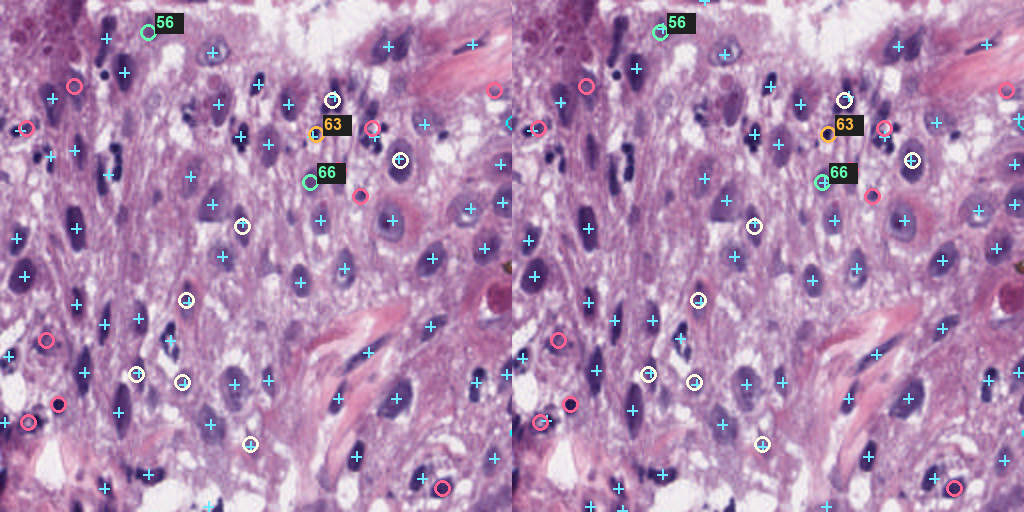
\includegraphics[width=\linewidth,height=.40\textheight,keepaspectratio]{assets/p31_image_1037_seed_19.png}
\captionof{figure}{P31 肺组织图像 1037，种子 19：左为对照，右为分组归一化。青色十字为预测中心；白、绿、橙、粉色圆圈分别表示共同找到、新方案找到、对照找到、共同漏检的内部死亡核；数字为标注对象编号。}
\raggedright

这张肺组织图像从 8/20 增至 9/20。对象 56 的标注中心在（行 16，列 74），最近预测点距离由 21.21 降至 2.24 像素；对象 66（91，155）由 19.65 降至 1.00。对象 63（67，158）则由 2.24 增至 20.52 像素，原有匹配消失。图中可观察到预测点出现和消失；距离按已保存的预测坐标计算。

\end{minipage}

\noindent

\begin{minipage}{\linewidth}\centering
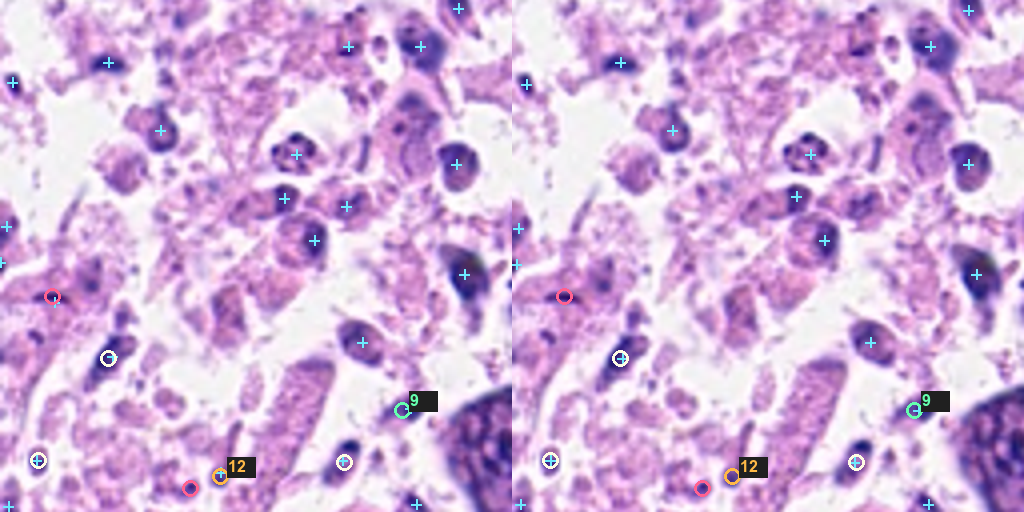
\includegraphics[width=\linewidth,height=.40\textheight,keepaspectratio]{assets/p31_image_776_seed_19.png}
\captionof{figure}{P31 结肠组织图像 776，种子 19：左为对照，右为分组归一化；青色十字为预测，白、绿、橙、粉色圆圈分别表示共同找到、新方案找到、仅对照找到、共同漏检。}
\raggedright

该图两组均找到 4/7 个目标，但对象发生交换：对象 9（205，201）由 4.12 移至 2.00 像素，进入匹配范围；对象 12（238，110）由 2.00 增至 61.40 像素，附近预测消失。种子 1 中这两个对象均新增匹配，图像由 4/7 增至 6/7。相同的图像总数可以包含不同对象的变化。

\end{minipage}

\noindent

\begin{minipage}{\linewidth}\centering
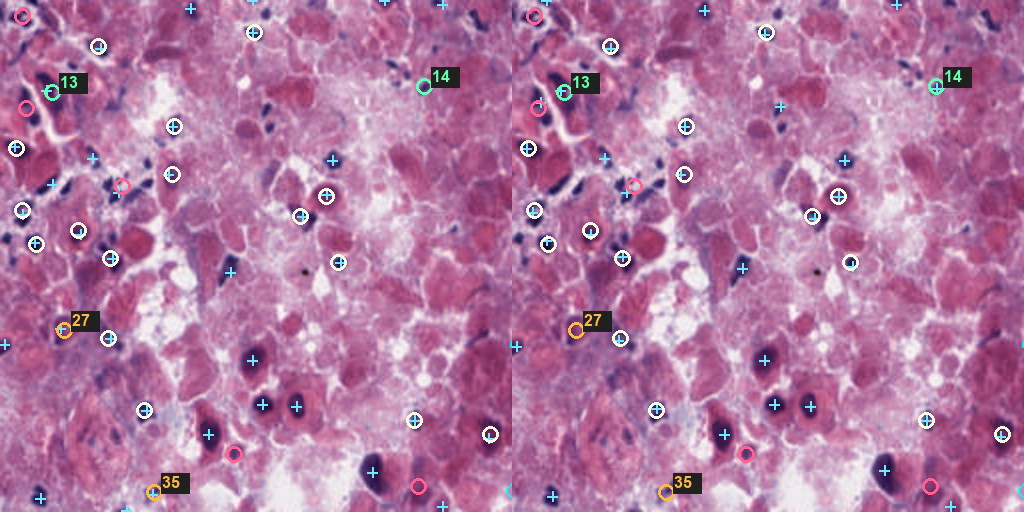
\includegraphics[width=\linewidth,height=.40\textheight,keepaspectratio]{assets/p31_image_1025_seed_1.png}
\captionof{figure}{P31 肺组织图像 1025，种子 1：左为对照，右为分组归一化；青色十字为预测，白、绿、橙、粉色圆圈分别表示共同找到、新方案找到、仅对照找到、共同漏检。}
\raggedright

这张图保持 18/25：面积 31 平方像素的对象 14（43，212）从最近点距离 41.98 降至 1.00，对象 13 从 3.16 降至 2.24；对象 27 和 35 则分别从 2.24、1.41 增至 21.59、41.01。原始图像和预测坐标显示新增与丢失，造成这些变化的模型内部过程需要另行测量。

\end{minipage}

\subsection{综合分析与资料来源}\label{ux7efcux5408ux5206ux6790ux4e0eux8d44ux6599ux6765ux6e90}

五轮都采用同一开发评估集及各自的同期对照。P27--P30
的变化显示，训练位置改变后，同一图像内既有新找到的细胞核，也有失去匹配的细胞核；P31
的检测头修改同样出现对象交换。P29 的两个种子均增加至少 13
个内部死亡核匹配，P30 的两个种子均增加至少 516 个全部细胞核匹配。P31
在训练图像上的检测率上升，同时两个种子的开发评估变化不同。各轮选择、两种子和匹配定义保持原实验记录。

所有组织图片来自固定样例的实际结果；图中青色十字表示预测中心，白、绿、橙、粉色圆圈分别表示两组共同找到、仅实验组找到、仅对照找到、两组均漏检的死亡细胞核。图内数字是标注对象编号。图像编号和坐标可在随附
evidence 目录中核对。P31 四次训练均完成，92
个小文件已按原保存清单核验；本报告附上用于图文的记录。数据出处、图像来源与复现方法见
NUMBER\_SOURCES.md 和 README.md。

\end{document}
